% NeurIPS-style arXiv preprint. Compile: tectonic -X compile main.tex
% Option [preprint] names authors and prints ``Preprint.'' in the footer.
% OpenReview: \usepackage{neurips_2026} (no preprint), drop identity from
% \author and \hypersetup. Do not use [final] until camera-ready.
\documentclass{article}

\usepackage[preprint]{neurips_2026}

\usepackage{amsmath,amssymb}
\usepackage{xcolor}
\usepackage{booktabs,array,tabularx}
\usepackage{graphicx}
\usepackage{placeins}
\usepackage{iftex}
\iftutex
  \usepackage{fontspec}
  % Filename lookup (arXiv xelatex). Bundled fonts/ is a local tectonic fallback;
  % TeX Live 2025 already ships these OTFs, so the arXiv zip omits fonts/.
  \IfFileExists{fonts/texgyretermes-regular.otf}{%
    \setmainfont{TeXGyreTermes}[
      Path = fonts/,
      Extension = .otf,
      UprightFont = texgyretermes-regular,
      BoldFont = texgyretermes-bold,
      ItalicFont = texgyretermes-italic,
      BoldItalicFont = texgyretermes-bolditalic
    ]
    \setmonofont{TeXGyreCursor}[
      Path = fonts/,
      Extension = .otf,
      UprightFont = texgyrecursor-regular,
      BoldFont = texgyrecursor-bold,
      ItalicFont = texgyrecursor-italic,
      BoldItalicFont = texgyrecursor-bolditalic,
      Scale = MatchLowercase
    ]
  }{%
    \setmainfont{texgyretermes-regular.otf}[
      BoldFont = texgyretermes-bold.otf,
      ItalicFont = texgyretermes-italic.otf,
      BoldItalicFont = texgyretermes-bolditalic.otf
    ]
    \setmonofont{texgyrecursor-regular.otf}[
      BoldFont = texgyrecursor-bold.otf,
      ItalicFont = texgyrecursor-italic.otf,
      BoldItalicFont = texgyrecursor-bolditalic.otf,
      Scale = MatchLowercase
    ]
  }
\fi
\usepackage{microtype}
\usepackage[hidelinks]{hyperref}

\hypersetup{
  pdftitle={When Can Language Models Join Without Lexical Cues?},
  pdfauthor={Pankaj Pandey},
  pdfsubject={Unique-Path Traversal versus End-to-End Accuracy under Path Ambiguity},
  colorlinks=false,
  pdfborder={0 0 0},
  breaklinks=true
}
\graphicspath{{./}}
\emergencystretch=2em

\title{When Can Language Models Join\\
Without Lexical Cues?\\
Unique-Path Traversal versus End-to-End Accuracy\\
under Path Ambiguity}

\author{%
  Pankaj Pandey \\
  Independent researcher, India \\
  \mbox{\texttt{mightypp.nits@gmail.com}} \\
  \url{https://github.com/pankajnits/oir}
}

\begin{document}
\maketitle

\begin{abstract}
We ask whether multi-hop answering over knowledge graphs needs readable
predicates, or only equality among identifiers.
\textbf{Opaque isomorphic reasoning (OIR)} is a measurement protocol: a
renaming $\sigma$ of entities and relations that we verify to be injective
on each instance's finite atom set, with no legend in the prompt.
HMAC-SHA256 is one generator of $\sigma$, not a cryptographic or privacy
primitive.

\textbf{Finding.} Unique sealed routes still join. Competing sealed routes
typically yield \texttt{UNKNOWN}, not the decoy.
With the start entity already named in the question, OpenAI opaque unique
is $32/32$; both-opaque unique is $32/32$ for Composer~2.5, OpenAI
\mbox{\texttt{gpt-5.6-sol}}, and Grok~4.5.
On the 26 city-valued \textsc{Wiki-H5} items, unique English, unique
opaque, and English two-path are $26/26$; named-arm opaque two-path is
$5/26$, $2/26$, $2/26$ across three draws of the unpinned alias
(August: \texttt{UNKNOWN} $21$, decoy $0$, selective accuracy $5/5$).
The $n{=}32$ lock is $6/32$: one extra gold on a non-city P159 HQ; both
decoys fall on items whose gold is one of those six, so the city slice has
decoy $0$.
A city-typed OpenAI freeze at $n{=}200$ (every HQ is Wikidata P31 city-like;
QIDs re-checked live) repeats the pattern: unique English/opaque $200/200$,
English two-path $199/200$, named-arm opaque two-path $38/200$
(Wilson $[0.14,0.25]$; \texttt{UNKNOWN} $151$, decoy $11$), plan $200/200$.
Exact-match under two sealed routes is strongly sensitive to prompt
surface form~\citep{sclar2024spurious}.
The largest OpenAI move at 512 tokens on cyclic decoys is case-id wording
(same-date 11~September: named-arm $5/32$ vs.\ hashed ids $20/32$; ARM line
kept). Later same-day draws are ${+}18$ and ${+}19$ items; August vs.\
September ${+}14$ mixes dates.
The ARM line at 4096/medium is non-monotonic and interacts with decoy type
(cyclic/constant: no ARM $25/27$, H5 $20/10$, K2 $30/26$).
English relation names restore OpenAI even with anonymous entities
(OE two-path $32/32$ vs.\ both-opaque $1/32$).
We score the answer node, not an emitted $(r_1,r_2)$.
Seals remove lexical cues; they are not a confidentiality proof.
\end{abstract}

\section{Introduction}

The scored Wikidata question is \emph{What city is the headquarters of the
company led by \mbox{Michael Eisner}?}
English unique-path context walks \texttt{works\_at} then
\texttt{headquartered\_in} to Burbank; that success may use English
predicates, or only equality among identifiers.
The two-path decoy is a second person$\to$company$\to$city route
(\texttt{partner\_of}/\texttt{located\_in}) to Kansas City.
Opaque two-path keeps the English question and entity names; those
predicates become HMAC tokens (\texttt{works\_at} $\mapsto$
\texttt{E334675310f05} on the scored Eisner item).
Figure~\ref{fig:spine} is the OpenAI named-arm relation-only $2{\times}2$.
On 26 city-valued items the unique-path cells are $26/26$ and named-arm
opaque two-path is $5/26$ (all misses \texttt{UNKNOWN}).
The $n{=}32$ bar is $6/32$: one extra gold on a non-city P159 HQ; both
decoys fall on items whose gold is one of those six.
A city-typed OpenAI $n{=}200$ freeze (Appendix~\ref{app:protocol}) is
unique-path $200/200$ and named-arm opaque two-path $38/200$.
Prompt-surface packing of the same graphs is Section~\ref{sec:header}
and Appendix~\ref{app:tokens}.

OIR measures whether a model can join after English predicate strings are
replaced by keyed opaque tokens. We write a 2-hop as two inferred maps
(only the answer node is scored): selection $q \mapsto (r_1,r_2)$ and
traversal $(v_0,r_1,r_2,G)\mapsto v_2$. Opacity does not, by itself, block
traversal. The question is when the prompt no longer maps query semantics
onto one of two sealed relation sequences. Putting the start entity in $q$
as the same atom as in $V$ (\textbf{start in $q$}) separates that question
from start-entity identification.

Each instance uses a keyed injective $\sigma$ on that instance's atom set
(HMAC-SHA256, 48-bit tokens; Section~\ref{sec:method}). The model emits the
answer node in the graph's namespace or \texttt{UNKNOWN}; recovering
$\sigma^{-1}$ is not scored. A written hop is an execution control. Matched
versus novel demonstrations test in-prompt reuse of shown seals.

OIR is a measurement protocol. HMAC renaming is the same family as PrivGemo's
entity map $\phi_Q$~\citep{privgemo2026}; we apply it to relation strings, which
that paper leaves as original or clustered schema labels. ``Lexical cues''
on the primary $2{\times}2$ means relation strings (entities stay English);
both-opaque is a separate ablation. English multi-hop scores should not be
read as evidence that the same join succeeds once predicates are sealed and
two same-type routes compete.

This paper reports: (i)~unique-route sealed execution with the start in $q$
and no written hop; (ii)~under two competing sealed routes the usual reply
is \texttt{UNKNOWN}, not the decoy, and exact-match moves with prompt
surface form (case-id wording; ARM line non-monotonic;
Section~\ref{sec:header});
(iii)~matched demonstrations restore shown seals, while novel seals do not.
What is new is the interaction of opacity with path ambiguity, not opacity
alone, and how large a prompt-surface move can be on the same sealed graph. Cited privacy KGQA
keeps relation strings as readable words~\citep{arog2025,privgemo2026,liu2026cor}.
We seal \emph{relation} strings, keep entities English, and cross that with
path ambiguity. Unique routes succeed; two competing same-type routes are
underspecified and packaging-sensitive (Table~\ref{tab:inventory}).

\begin{figure}[t]
\centering
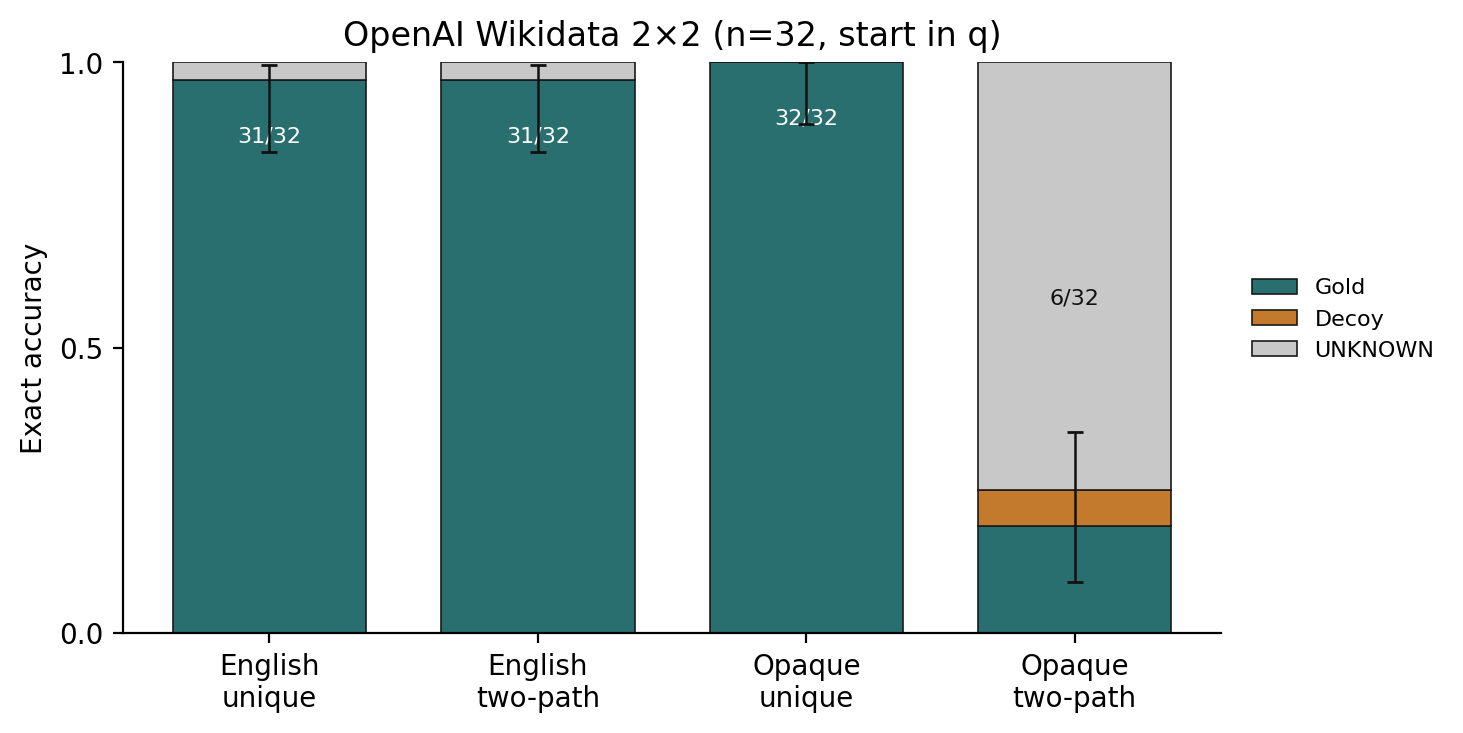
\includegraphics[width=0.92\linewidth]{fig1_matched_2x2.png}
\caption{OpenAI \textsc{Wiki-H5} on Wikidata ($n{=}32$, start in $q$;
relation-only). Stacked bars are gold / decoy / \texttt{UNKNOWN};
whiskers are Wilson 95\% intervals on exact match (item-level, one August
draw).
English unique/two-path $31/32$; opaque unique $32/32$; named-arm opaque
two-path $6/32$ (mostly \texttt{UNKNOWN}).
City-valued subset: unique-path $26/26$, opaque two-path $5/26$
(decoy $0$).
Prompt-surface ablations of the same graphs are Section~\ref{sec:header},
not plotted.}
\label{fig:spine}
\end{figure}

\section{Related Work}

Think-on-Graph and Reasoning-on-Graphs select the next readable
relation~\citep{sun2024tog,luo2024rog}. Ciphered ICL is not path ambiguity on a
labeled graph~\citep{fang2025ciphers,guo2025ciphered}.
GSM-Symbolic swaps entity names in English math~\citep{mirzadeh2025gsm};
2WikiMultihopQA is a readable multi-hop control~\citep{ho2020constructing}.

ARoG anonymizes \emph{entities} while relations stay the retrieval
language~\citep{arog2025}. PrivGemo HMAC-seals entities ($\phi_Q$, e.g.\
\texttt{ent\_17}); relations stay original labels or clustered schema words,
not keyed opaque tokens, and a local Hand answers on the raw graph after a
remote Brain ranks retrieved paths (CWQ $67\%\to 59\%$; WebQSP
$75\%$)~\citep{privgemo2026}.
CoR explores readable relations because entities often have no semantics
beyond opaque IDs --- the OE hide-set, not relation-only
\textsc{Wiki-H5}~\citep{liu2026cor}.
\citet{tang2023semantic} find LLMs fail when relation names are replaced by
symbols (\texttt{r1}) and rules must carry deduction; OpenAI unique-path
opaque $32/32$ is the complementary case: sealed relations still traverse
when topology fixes the route.
\citet{guo2025twohop} report collapse to random guessing among end entities
when distractor two-hops have other sources. Named-arm Wiki-H5 opaque
two-path, with \texttt{UNKNOWN} allowed, is abstention rather than guessing
(OpenAI decoy $2/32$, \texttt{UNKNOWN} $24/32$).
Section~\ref{sec:header} shows that this is a named-arm fact for at least
Grok: no-ARM opaque commits are near chance.
A forced-choice arm is not
in this evaluation (Section~\ref{sec:limitations}) and would put those
protocols on the same scale.
OIR withholds retrieved paths on the free arms (Table~\ref{tab:diff}).
The primary cell seals relations while entities stay English; both-opaque is
a separate ablation.

Chain-of-thought and Text-to-SQL externalize plans over
English~\citep{wei2022cot,yu2018spider}.
We ask a behavioral question: can a pretrained model join when the relation
vocabulary is freshly randomized and no plan is given? A sealed plan is then
an execution upper bound.
NLGraph and Talk like a Graph encode graphs without readable typed
predicates~\citep{wang2023nlgraph,fatemi2024talk}; OIR starts from a labeled
KG and removes only the relation lexicon.
ARM headers are a prompt-surface feature~\citep{sclar2024spurious}.
Symbol tuning, binding-ID analyses, and compositional-limit studies change
the labels or the task~\citep{wei2023symbol,feng2024binding,dziri2023faith}.
OIR holds the join, hop length, graph size, and question template fixed and
replaces relation strings; OpenAI unique-path opaque traversal stays at
$32/32$, so that removal withdraws the cue that would otherwise select
between routes rather than blocking execution.

\begin{table}[t]
\centering
\small
\setlength{\tabcolsep}{3.2pt}
\begin{tabular}{@{}>{\raggedright\arraybackslash}p{1.55cm}
                 >{\raggedright\arraybackslash}p{2.55cm}
                 >{\raggedright\arraybackslash}p{2.85cm}
                 >{\raggedright\arraybackslash}p{2.85cm}@{}}
\toprule
Work & Hidden & Remote task & Join under opacity \\
\midrule
ICL CIPHERS & substitution text & ICL task accuracy (bijection inferred) & ICL tasks \\
ARoG & entities; relations readable; topic names in $q$ & retrieve $+$ generate (relations, concepts) & privacy KG-RAG \\
PrivGemo & entities (HMAC); relations original or clustered schema words & rank retrieved paths; local plaintext answer & privacy KG-RAG \\
CoR & opaque entity IDs; relations readable & relation-centric exploration & KGQA \\
\textbf{OIR} & relations (primary $2{\times}2$); entities too (ablation); one join or none & emit graph-namespace answer (no local decode) & selection vs.\ traversal \\
\bottomrule
\end{tabular}
\caption{Related protocols. PrivGemo HMAC-seals entities; relations remain
original or clustered schema labels. OIR sends one graph and scores the answer
token from the same model.}
\label{tab:diff}
\end{table}
\FloatBarrier

\section{Problem Formulation}
\label{sec:problem}

Let $G=(V,R,T)$ be a labeled multi-relational graph
($T\subseteq V\times R\times V$) and $q$ a natural-language or programmatic
query with answer $a\in V$. A \textbf{seal} $\sigma$ is a keyed map from
entity and relation strings to opaque tokens that we verify to be injective
on the finite normalized atom set of each evaluation instance. We reject any
instance where two distinct raw atoms normalize to the same string.
Truncated HMAC-SHA256 is not injective over $\{0,1\}^{\ast}$; we use 48-bit
truncation because that width is injective on our small per-instance atom
sets, not as a cryptographic bound. On the scored Wikidata $2{\times}2$
instances, no HMAC collision was observed. HMAC is computed from the
normalized atom string; entity and relation types are not domain-separated,
so identical plaintext yields the same token regardless of type. On each
scored evaluation instance the normalized entity strings and relation
strings are disjoint, so no entity is identified with a relation. The model
receives $G$ or $\sigma(G)$ and a query form built from $\sigma$ (or from
English, depending on the arm) and must return the answer node in that
namespace; recovering $\sigma^{-1}$ is not scored. Sealing is deterministic
\emph{given the instance key}; the same plaintext need not map to the same
token across prompts.

A 2-hop join factors as two maps we measure separately:
\begin{align}
\text{selection:}&\quad (q,G,\mathcal{C})\mapsto (r_1,r_2), \label{eq:sel}\\
\text{traversal:}&\quad (v_0,r_1,r_2,G)\mapsto v_2. \label{eq:trav}
\end{align}
In general, traversal is set-valued
($\tau_G\colon V\times R\times R\to 2^V$);
we evaluate only instances for which $|\tau_G(v_0,r_1,r_2)|=1$ for the gold
plan (and, on two-path items, for the decoy plan as well), so each scored
route has a unique tail. Uniqueness is per plan, not ``one answer in $G$.''
We write $q\mapsto(r_1,r_2)$ when $G$ and prompt context $\mathcal{C}$ are
held fixed. A sealed join plan supplies $(r_1,r_2)$ and tests~\eqref{eq:trav}.
Unique-path items with $v_0$ already in $q$ also test~\eqref{eq:trav} when
topology leaves only one route. Free sealed English tests~\eqref{eq:sel}
then~\eqref{eq:trav} together. Dual-path items hold $G$ fixed, give two
complete routes from $v_0$, and vary whether demonstrations expose the gold
seals. The CEO free-English arm does \emph{not} put $v_0$ in $q$ as a single
graph atom (the question is hashed piecewise), so it is not a pure test
of~\eqref{eq:sel}.

A 2-hop is \emph{structurally executable} when $(r_1,r_2)$ is given, or when
topology leaves only one 2-hop from a start already in $q$. The prompt
\emph{explicitly maps} query semantics onto one relation sequence when it
contains English predicates, a legend, or demonstrated seals. When two
complete routes exist and relation tokens are arbitrary HMAC strings with no
such mapping supplied, selection is \emph{unsupported by explicit cues}
under this construction. Residual statistical structure can remain (token
form, order, HMAC vs.\ permutation rates); we do not claim mathematical
unidentifiability. Without an external semantic-to-symbol map, the gold
route is not explicitly identifiable from the sealed two-path graph alone;
any successful selection must rely on residual statistical cues or
information supplied elsewhere in the prompt. Low exact-match is therefore
unsurprising when the prompt provides no explicit mapping; it is not
evidence that traversal failed. Dual-path separates those cases: in-prompt
reuse of demonstrated relation-seal correspondences restores end-to-end
accuracy; novel seals receive no such mapping. Models may abstain
(\texttt{UNKNOWN}) rather than guess. That is selective
prediction~\citep{elyaniv2010selective,geifman2017selective}, studied in
language models as calibration and
abstention~\citep{kadavath2022know,wen2025abstention}: coverage is the
fraction of items with a non-\texttt{UNKNOWN} parse, and selective accuracy
is exact match among those items, not a forced-choice among the two routes.

After sealing, the Eisner unique-path CONTEXT is
\texttt{Michael\_Eisner | E334675310f05 | The\_Walt\_Disney\_Company} then
\texttt{The\_Walt\_Disney\_Company | Eac04fab538ca | Burbank}
(12-hex tokens; entities remain English on the primary $2{\times}2$).

We use five measurement arms.
\textbf{Readable English} is the baseline (start in $q$; names and
predicates unsealed).
\textbf{Unique opaque} has one 2-hop and no plan: execution when topology
uniquely determines the route.
\textbf{Two-path opaque} has two same-type 2-hops and no plan: end-to-end
behavior when two complete routes compete and the prompt supplies no
semantic-to-symbol map; the scored output is the answer node or
\texttt{UNKNOWN}, not $(r_1,r_2)$.
\textbf{Sealed join plan} writes $(r_1,r_2)$ over $\sigma$-atoms (execution
control); a non-LLM router saturates on the same sequence.
\textbf{Free sealed English} seals the question and graph with no plan and
no legend. On CEO, the question is hashed piecewise, so the full person atom
in $G$ typically does not appear in $q$ (confounded; not the matched
factorial).
Additional scaffolds (name/key legends, sealed demonstrations) appear as
ablations.

The scored output on every free arm is that answer node (plaintext city when
entities stay English; $\sigma(a)$ when entities are sealed) or
\texttt{UNKNOWN}. We infer whether selection was supported from those
end-to-end outcomes and from controls (unique topology, written hop, matched
vs.\ novel seals); we do not score an emitted $(r_1,r_2)$. Throughout,
``selection failure'' names that inference about the latent $(r_1,r_2)$
stage; we do not observe the pair.

\section{Method}
\label{sec:method}

\paragraph{Seal recipe.}
Normalize each atom: strip; collapse whitespace to \texttt{\_}; map other
non-alphanumeric characters (except underscore, period, hyphen) to
\texttt{\_} using the ASCII class \verb|[A-Za-z0-9_.-]| (so
\texttt{Z\"{u}rich}$\mapsto$\texttt{Z\_rich}; pure CJK keeps Unicode);
truncate to 64; empty maps to \texttt{EMPTY}.
The CEO JSON already deleted diacritics upstream. Distinct raw
atoms must normalize to distinct strings. Tokens are HMAC-SHA256 over UTF-8
bytes with a per-item 16-byte key; the token is \texttt{E} plus the first
6 digest bytes as 12 hex digits. HMAC is keyed renaming, not a security
mechanism: 48-bit truncation is instance-wise injective on our small atom
sets. On the scored Wikidata $2{\times}2$ graphs, normalization and HMAC
produced no collisions among prompt atoms. The intervention removes lexical
semantics and also changes token-level surface statistics; permutation and
alphanumeric generators assess robustness to that latter variation
(Table~\ref{tab:tokens}). The atom \texttt{Michael Eisner} normalizes to
\texttt{Michael\_Eisner}, so those two strings receive the same seal.
Hashing the question token-by-token does not reconstruct that graph atom,
which is the missing-start failure a name-binding wrapper is designed to
prevent. Reported opaque cells are performance under this keyed HMAC
construction, not a claim that every opaque identifier distribution yields
the same rate.

\paragraph{Matched $2{\times}2$ (start in $q$).}
\label{par:fact2x2}
The $n{=}32$ suite is a seeded random sample of 32 of 73 Wikidata-derived CEO
records (\texttt{random.Random(20260821).sample};~\citealp{vrandecic2014wikidata}),
not a published CEO benchmark and not a hand-picked subset.
Each instance is 4 triples (unique-path: 6 entities with a disconnected
decoy island; two-path: 5 entities sharing the start). The gold two-hop
uses \texttt{works\_at} then the headquarters relation; the question says
``led by''. The competing two-path route is synthetic
(\texttt{ambig\_edges} attaches record $i{+}1$'s company/HQ under
\texttt{partner\_of}/\texttt{located\_in}; not a Wikidata fact; decoy HQ
pool $=$ gold HQ pool). To isolate relation selection from start-entity
identification we keep the start string in the question and hold hop
length, template, and graph size fixed. Two factors vary: relation labels
(English vs.\ HMAC) and topology (one 2-hop from the start vs.\ two).
Tails are intended as the same type; Wikidata P159 was not filtered
(buildings/stations/a street among gold HQs; both OpenAI opaque two-path
decoys sit on city/non-city pairs; Appendix~\ref{app:protocol}).
On Wikidata two-path graphs both intermediates are companies
(\texttt{works\_at}/\texttt{headquartered\_in} vs.\
\texttt{partner\_of}/\texttt{located\_in}).
In the primary run the gold 2-hop is listed before
the decoy 2-hop in CONTEXT; that order is the same in the English and opaque
arms. A shuffled listing of the same 32 graphs and HMAC keys (16 gold-first,
16 decoy-first) is a robustness check on a later endpoint snapshot
(Appendix~\ref{app:protocol}): English two-path $29/32$, opaque two-path
$5/32$ (\texttt{UNKNOWN} $25/32$, decoy $1/32$, other $1/32{=}\texttt{Lod}$). Opaque gold-first is $3/16$
vs.\ decoy-first $2/16$ (decoy $0/16$ vs.\ $1/16$): putting the decoy
route first does not raise the decoy rate.

The primary two-path prompt is a single user message:
\begin{quote}
\small
\texttt{MODEL UNDER TEST. Read ONLY this file. Use CONTEXT only. No other files.}\\
\texttt{Format: ANSWER\_PLAIN[\ldots]: <city\_or\_UNKNOWN>}\\
\texttt{ARM OPAQUE\_AMBIG: opaque relations, English entities;}\\
\texttt{two 2-hops from start.}
\end{quote}
It does \emph{not} contain the equality-recipe line
(Appendix~\ref{app:recipe}).
The format token is \texttt{<city\_or\_UNKNOWN>}, but six gold HQs are not
cities (Appendix~\ref{app:protocol}). A model that obeys the format on those
items must emit \texttt{UNKNOWN}. The 26 city-valued items are the primary
report in Section~\ref{sec:fact2x2}; the $n{=}32$ hash-pinned cell is the
robustness note and the lockfile.
OpenAI English two-path is $31/32$ under that CONTEXT-only instruction, so the
line does not by itself force abstention.
Readable names (Eisner, Burbank) still leave OpenAI at \texttt{UNKNOWN}
$24/32$ on opaque two-path: either parametric HQ is treated as
inadmissible, or the verb does not map onto one seal.
We cannot separate those readings here (Section~\ref{sec:limitations}).
The CEO three-arm decoy 2-hop begins at a different person; it is not the
matched two-path factorial.

\paragraph{Further constructions.}
The relation-only factorial keeps entities English. A second isolation suite
on the same 32 CEO records seals entities, relations, or both, always with
the start token in $q$. Opaque-entity / English-relation (OE) is the
ARoG-like cell: readable predicates, anonymous nodes. Both-opaque
(\textsc{Wiki-OO}) seals entities \emph{and} relations; it is a
complementary ablation, not the primary relation-only $2{\times}2$. Readable
entity names therefore leave residual pretrained world knowledge as a
possible cue; both-opaque is not a substitute for synthetic identifiers.

WikiMovies facts are sampled from the public MetaQA movie
KB~\citep{miller2016wikimovies,zhang2018metaqa}.
\textsc{Movie-A32} and \textsc{Movie-A100} leave English verbs such as
\emph{directed} in $q$;
\textsc{Movie-B} hashes question atoms except the bracketed start entity.
We exclude a genre-vs-language variant because object type would bypass
relation selection. This is not an evaluation on the official MetaQA 14K
test split. Dual-path holds $G$ fixed with two complete 2-hop routes and
varies whether demonstrations expose the gold seals
(Appendix~\ref{app:dual}).

\paragraph{Scoring.}
The format asks for one answer token in the graph's namespace or
\texttt{UNKNOWN}. Primary metric: exact match (\texttt{UNKNOWN} is a miss).
Scored \texttt{UNKNOWN} on Wiki-H5/Wiki-OO is an explicit \texttt{UNKNOWN}
line. Dual and some no-hop OpenAI cells stored empty completions as
\texttt{UNKNOWN}. On two-path arms we also report decoy
and \texttt{UNKNOWN} rates (Table~\ref{tab:threeway}).
Wilson 95\% intervals use $z{=}1.96$~\citep{wilson1927}
($0/32 \Rightarrow [0.00,0.11]$;
$6/32 \Rightarrow [0.09,0.35]$;
$32/32 \Rightarrow [0.89,1.00]$).
Those intervals treat the 32 items as Bernoulli trials on a single draw;
they are not a generation-variance interval. OpenAI \textsc{Wiki-H5} $k{=}3$
(August lock plus two later draws) is Section~\ref{sec:fact2x2}.
On the OpenAI Wikidata $2{\times}2$, English two-path is correct and opaque
two-path is not on $25$ of $32$ paired items, and the reverse never occurs
(McNemar exact two-sided complete-case $p{=}5.96{\times}10^{-8}$;~\citealp{mcnemar1947}).
That is the two-path paired contrast, not an interaction test, and it
largely measures removing the cue that made one sealed route identifiable.
The empirical content is the response mode (\texttt{UNKNOWN} vs.\ decoy)
and prompt-surface packing (Section~\ref{sec:header}).
That $p$ clears $0.001$ (confirmatory McNemar only).
\textbf{Isolation} means one quiz per file with gold answers stored outside
the model-visible prompt (stricter than multi-quiz \textbf{batch} files).
Isolation $n{=}32$ uses one quiz per file and a per-item HMAC. Cells marked
\textbf{n.r.} were not evaluated; we never impute them as zeros.
\emph{Mid-hop error} means the model emits the sealed mid-hop company token
instead of the headquarters answer.

\paragraph{Models.}
The primary family is OpenAI
\mbox{\texttt{gpt-5.6-sol}} (hereafter OpenAI). Composer~2.5 and Grok~4.5
are a robustness note on the same quiz files, not a ranking
(Table~\ref{tab:threeway}). Secondary
packaging probes additionally use an unversioned Claude endpoint
(Anthropic model id not stored; Appendix~\ref{app:middleware}).
\texttt{gpt-5.6-sol} is the GPT-5.6 Sol Chat Completions endpoint (Sol is
the flagship-equivalent tier of the GPT-5.6 family;
\url{https://developers.openai.com/api/docs/models/gpt-5.6-sol}).
OpenAI cells use that API with no tools, temperature
omitted because that family rejects temperature~$0$
(\texttt{max\_completion\_tokens} 512). The runner does not pass
\mbox{\texttt{reasoning\_effort}} and used the unpinned alias
\texttt{gpt-5.6-sol}; the August lock stores the parsed answer, not the
API \texttt{model} string. $k{=}3$ OpenAI draws (August lock plus two
15~September~2026 draws with JSON sidecars that \emph{do} store
\texttt{returned\_model}) are reported in Section~\ref{sec:fact2x2}.
Composer~2.5 and Grok~4.5 ran through Cursor's agent SDK
on the same quiz files, with a reply-only preamble OpenAI never received.
Tools, retry, and empty-reply handling are not equated (OpenAI locked empty
completions as \texttt{UNKNOWN}). Unique-path opaque stays high on all three
(Composer $27/32$, OpenAI $32/32$, Grok $30/32$): those SDK cells still
execute unique-path joins. Named-arm difference-in-differences (DiD) is
most readable for OpenAI
(Grok English two-path $4/32$ vs.\ English, no ARM, hashed ids $24/32$;
Section~\ref{sec:header}).
Unique both-opaque $32/32$ is the three-family traversal cell. Isolation
quizzes (\texttt{runs/}) and locked exact-match scores (\texttt{results/})
are at \url{https://github.com/pankajnits/oir}. Inference settings are
Appendix~\ref{app:protocol}.

\FloatBarrier
\section{Results}
\label{sec:results}

Table~\ref{tab:inventory} names the cells. \textsc{Wiki-H5} is the Wikidata
CEO relation-only $2{\times}2$ with the start already in $q$ (OpenAI
primary; Composer/Grok are a different harness).
\textsc{Wiki-OO} seals entities \emph{and} relations on the same graphs;
OE seals entities only.
\textsc{Movie-A32} is WikiMovies $n{=}32$ with English verbs still in $q$;
\textsc{Movie-A100} is the $n{=}100$ version; \textsc{Movie-B} hashes those
verbs except the start.
Header$\times$decoy is the same 32 people with hashed case ids, crossing the
ARM line with cyclic vs.\ constant decoys (Section~\ref{sec:header}).
\textsc{Movie-B} is a cross-dataset check, not a resampling of
\textsc{Wiki-H5}. Packaging probes ($n{\le}16$) are
Appendix~\ref{app:packaging} and do not bear on the $2{\times}2$.

\begin{table}[htbp]
\centering
\small
\setlength{\tabcolsep}{3.0pt}
\begin{tabular}{@{}llllll@{}}
\toprule
ID & Dataset & Condition & $n$ & Models & Scored \\
\midrule
\textsc{Wiki-H5} & Wikidata CEO & rel-only $2{\times}2$, start in $q$ & 32 & OpenAI (primary) & node \\
\textsc{Wiki-H5-200} & Wikidata CEO, city P31 & same $2{\times}2$, QID freeze & 200 & OpenAI & node \\
Header$\times$decoy & same 32 people & ARM line $\times$ decoy, hashed ids & 32 & 3 families & node \\
Header$\times$decoy-200 & same 200 people & ARM $\times$ decoy, hashed ids & 200 & OpenAI & node \\
\textsc{Wiki-OO} & same graphs & both-opaque & 32 & 3 families & $\sigma(a)$ \\
\textsc{Wiki-OO-200} & n=200 freeze & both-opaque & 200 & OpenAI & $\sigma(a)$ \\
\textsc{Wiki-Shuf} & same two-path & listing order & 32 & OpenAI & city \\
\textsc{Movie-A32} & WikiMovies & actor$\to$movie$\to$dir vs writer & 32 & 3 models & person \\
\textsc{Movie-A100} & WikiMovies & same hops; verbs in $q$ & 100 & OpenAI & person \\
\textsc{Movie-A200} & WikiMovies & n=100 prefix + 100 new actors & 200 & OpenAI & person \\
\textsc{Movie-B} & WikiMovies & same hops; verbs hashed & 100 & OpenAI & person \\
\textsc{Movie-B200} & WikiMovies & Condition B on n=200 freeze & 200 & OpenAI & person \\
\textsc{Dual} & WikiMovies/synth & matched vs.\ novel demos & 32 & 3 models & $\sigma(a)$ \\
\textsc{Dual-200} & WikiMovies n=200 & matched vs.\ novel & 200 & OpenAI & $\sigma(a)$ \\
\textsc{CEO-NL} & Wikidata CEO & piecewise $q$, no plan & 32 & 3 models & $\sigma(a)$ \\
\textsc{CEO-NL-200} & n=200 freeze & piecewise $q$, no plan & 200 & OpenAI & $\sigma(a)$ \\
\bottomrule
\end{tabular}
\caption{Cell inventory, listed before results.
\textsc{Wiki-H5} is the OpenAI discovery (Composer/Grok in
Table~\ref{tab:threeway}, not a ranking).
Header$\times$decoy and the case-id contrast are Section~\ref{sec:header}.
Scored output is the answer node; six P159 golds
are not cities, so the city-valued $n{=}26$ slice is the $n{=}32$ headline
(Appendix~\ref{app:protocol}).
\textsc{Wiki-H5-200} is a separate city-typed QID freeze (OpenAI).
A32/A100/B share the actor$\to$movie$\to$director vs.\ writer template;
A100 Condition~A uses a thinner ARM than A32. Isolation cells use per-item HMAC; batch
three-arm $n{=}12$/$n{=}24$ share one key per file.}
\label{tab:inventory}
\end{table}

\subsection{Opacity \texorpdfstring{$\times$}{x} path ambiguity}
\label{sec:fact2x2}

\textsc{Wiki-H5} holds the start string in $q$ and varies only relation
lexicality (English vs.\ HMAC) and the number of 2-hops from that start
(one vs.\ two). OpenAI is the primary family. Composer~2.5 and Grok~4.5
are Table~\ref{tab:threeway} robustness, not a ranking: they used Cursor's
agent SDK with a preamble OpenAI never received.

Lead with the response mode, then the rate.
On unique sealed routes OpenAI executes (opaque unique $32/32$; plan on
the two-path graph $32/32$).
On competing sealed routes the usual named-arm reply is
\texttt{UNKNOWN}, not the decoy.
The headline cell is the 26 city-valued items, where the format token
\texttt{<city\_or\_UNKNOWN>} is well-posed:
unique English, unique opaque, and English two-path are $26/26$;
named-arm opaque two-path is $5/26$, $2/26$, $2/26$ across three draws of
the unpinned alias ($k{=}3$ below).
August (draw~1): \texttt{UNKNOWN} $21$, decoy $0$, selective accuracy $5/5$;
McNemar $21$ vs.\ $0$, $p{=}9.54{\times}10^{-7}$;~\citealp{mcnemar1947}.
Unique-path $\Delta_{\mathrm{opq}}$ is $0/26$.

The hash-pinned $n{=}32$ lock is the robustness note, not the headline.
English unique $31/32$, English two-path $31/32$, opaque unique $32/32$,
named-arm opaque two-path $6/32$ (\texttt{UNKNOWN} $24$, decoy $2$).
Both decoys fall on items whose gold is one of the six non-city P159 HQs
(items 27 and 31; Appendix~\ref{app:protocol}); a model that obeys the city
format on those items is forced toward \texttt{UNKNOWN} or a type error.
Wilson 95\% on the August $n{=}32$ lock (item-level, one draw):
$32/32 \Rightarrow [0.89,1.00]$,
$31/32 \Rightarrow [0.84,0.99]$,
$6/32 \Rightarrow [0.09,0.35]$.
On the city slice of that same draw,
$5/26 \Rightarrow [0.09,0.38]$.
Figure~\ref{fig:spine} plots the $n{=}32$ OpenAI $2{\times}2$.

\paragraph{City-typed $n{=}200$ (OpenAI).}
The $n{=}32$ source file has 73 CEO rows and six non-city P159 golds.
\textsc{Wiki-H5-200} is a new freeze: 200 unique people and companies,
HQ frequency capped at 3, every HQ an instance of a city-like Wikidata
class, person/company/HQ QIDs stored, and all 200 P169+P159+P31 triples
re-checked live against the Query Service
(\texttt{wikidata\_ceo\_hops\_n200.json}).
It does not overwrite the $n{=}32$ lock.
OpenAI named-arm: unique English and unique opaque $200/200$, English
two-path $199/200$, opaque two-path $38/200$ (\texttt{UNKNOWN} $151$,
decoy $11$; Wilson $[0.14,0.25]$), plan $200/200$.
The $38/200$ rate sits inside the $n{=}32$ Wilson band for $6/32$.
Same-date hashed-id H5-cyclic at 512 tokens is $134/200$ vs.\ named-arm
$38/200$ (ARM line kept): the case-id gap is not an $n{=}32$ artifact.
Header$\times$decoy at 4096/medium on the same 200 people
(Table~\ref{tab:headerdecoy200}): cyclic/constant no ARM $174/151$,
H5 $129/44$, K2 $179/144$; English no ARM cyclic $197/200$.
H5 cyclic vs.\ constant McNemar $95$ vs.\ $10$, $p{=}1.6{\times}10^{-18}$;
no-ARM $30$ vs.\ $7$, $p{=}1.9{\times}10^{-4}$.
Both-opaque two-path is $12/200$ (unique $200/200$; OE two-path $200/200$).
Listing-order shuffle: opaque two-path $59/200$ (gold-first $25/100$,
decoy-first $34/100$).
CEO-NL free sealed English $0/200$ with plan $200/200$.
WikiMovies Condition~A $122/200$ two-path (unique $200/200$);
Condition~B $7/200$; Dual novel $2/200$ vs.\ matched $200/200$.
Condition~A $n{=}200$ uses the Wiki-H5 topology ARM line, not the A100
banner \texttt{ARM OPAQUE\_AMBIG n=100}, so $122/200$ is not a resample of
$96/100$.
$n{=}200$ is OpenAI-only; three-family cells stay at $n{=}32$.

Let $\Delta_{\mathrm{opq}}$ be opaque minus English exact-match on $n{=}32$.
Unique path: $\Delta_{\mathrm{opq}}=+1/32$ ($32/32$ vs.\ $31/32$), one
non-city miss.
Two-path: $\Delta_{\mathrm{opq}}=-25/32$ ($6/32$ vs.\ $31/32$).
The descriptive difference-in-differences is $-26/32$.
Section~\ref{sec:method} already notes that the gold route is not
explicitly identifiable from the sealed two-path graph, so that DiD
substantially measures removing the disambiguating cue.
The paired count remains: 25 items English-correct and opaque-wrong, 0
reverse (McNemar exact two-sided $p{=}5.96{\times}10^{-8}$;~\citealp{mcnemar1947}).
Opacity is not a randomized within-item treatment.
Wilson intervals treat items as independent Bernoulli trials, which the
cyclic decoy construction slightly violates (Appendix~\ref{app:protocol}).
An optional sign-flip of the per-item interaction contrast
is Appendix~\ref{app:signflip} (same numerical $p$, different test).

\paragraph{OpenAI $k{=}3$.}
Every August cell is one sample; temperature is omitted.
The $k{=}3$ protocol reuses that August lock as draw~1 and adds two
15~September~2026 draws on the same quiz files, same alias, 512 completion
tokens, sidecars storing \texttt{returned\_model}
(\texttt{factorial\_2x2\_iso\_gpt56k3r2.json},
\texttt{factorial\_2x2\_iso\_gpt56k3r3.json}).
Those later draws are a new snapshot of the unpinned alias, not a
resample of a pinned checkpoint, so they do not deliver a
generation-variance interval.

Named-arm opaque two-path is $6/32$, $3/32$, $3/32$
(city-valued $5/26$, $2/26$, $2/26$).
Draws~2 and~3 are the same day and give identical counts.
The same shape appears in Composer ($10$, $7$, $6$) and Grok ($1$, $0$, $0$):
August is highest in all three families.
Within a snapshot the counts barely move; the August-to-September gap looks
like drift in the served alias and moves all three families the same
direction on this cell.
The later draws stay well below the hashed-id H5-cyclic rate ($20$--$22/32$).
Unique opaque is $32/32$, $31/32$, $32/32$; English two-path is $31/32$,
$30/32$, $30/32$; plan is $32/32$ on every draw.
A separate 11~September snapshot of named-arm opaque two-path only
(\texttt{gpt56sep}) is $5/32$ (one \texttt{NO\_OUTPUT}) and is not one of
the three draws; with hashed-id H5-cyclic $20/32$ that day it is the
same-date case-id pair in Section~\ref{sec:header}.

This pattern is \emph{not} a universal three-family exact-match rate.
Unique-path opaque stays high on all three. On named-arm opaque two-path
the usual reply is \texttt{UNKNOWN}, not the decoy. Named-arm English two-path is OpenAI
$31/32$, Composer $26/32$, Grok $4/32$ (\texttt{UNKNOWN} $28$;
English, no ARM, hashed ids $24/32$): a packaging$\times$family effect, not a ranking
(Section~\ref{sec:header}).
Opaque unique remains high (Composer $27/32$, Grok $30/32$);
named-arm opaque two-path drops ($10/32$, $1/32$); a written hop recovers
($28/32$, $32/32$). Exact-match alone hides the behavior: opaque two-path
is mostly \texttt{UNKNOWN}, not decoy. Coverage is the fraction of items with
a non-\texttt{UNKNOWN} parse; selective accuracy is exact match among those
items~\citep{elyaniv2010selective,geifman2017selective}.
Two-path coverage / selective accuracy (named-arm):
OpenAI English $31/32$, $31/31$ and opaque $8/32$, $6/8$;
Composer English $26/32$, $26/26$ and opaque $10/32$, $10/10$;
Grok English $4/32$, $4/4$ and opaque $1/32$, $1/1$.
A forced uniform guess among two routes would be $1/2$; that is not the
relevant null once \texttt{UNKNOWN} is allowed.
Composer English two-path $26/32$ is $26/26$ on cities (all six misses are
those P159 golds). Grok named-arm English two-path is $4/26$: that
named-arm abstention is not a format artifact.
Composer named-arm opaque two-path, same Cursor preamble as the August lock:
$10/32$, $7/32$, $6/32$.
Grok: $1/32$, $0/32$, $0/32$.
Unique-path cells were not resampled for those families.

On the same graphs under two other opaque generators, unique-path accuracy
exceeds two-path accuracy (permutation $31/32$ vs.\ $15/32$; alphanumeric
$29/32$ vs.\ $12/32$; Table~\ref{tab:tokens}). Direction agrees across three
generators; the two-path \emph{rate} is not invariant.

\begin{table}[t]
\centering
\small
\setlength{\tabcolsep}{3.5pt}
\begin{tabular}{@{}lccc@{}}
\toprule
Wikidata named-arm (iso.\ $n{=}32$) & OpenAI & Composer~2.5 & Grok~4.5 \\
\midrule
English, unique & $31/0/1/0$ & $29/0/2/1$ & $32/0/0/0$ \\
English, two paths & $31/0/1/0$ & $26/0/6/0$ & $4/0/28/0$ \\
Opaque, unique & $32/0/0/0$ & $27/0/3/2$ & $30/0/2/0$ \\
Opaque, two paths & $6/2/24/0$ & $10/0/22/0$ & $1/0/31/0$ \\
Opaque two paths $+$ plan & $32/0/0/0$ & $28/0/3/1$ & $32/0/0/0$ \\
\bottomrule
\end{tabular}
\caption{Four-way outcomes: gold / decoy / \texttt{UNKNOWN} / other wrong token.
OpenAI is the primary family (August lock; $k{=}3$ in the surrounding text).
Composer~2.5 and Grok~4.5 used Cursor's agent SDK with a reply-only preamble
OpenAI never received; this table is not a ranking.
On this table \texttt{UNKNOWN} is an explicit \texttt{UNKNOWN} line
(missing/unparsed $0$; both-named $0$).
Composer ``other'' is truncated gold \texttt{Lod} (English unique, opaque
unique, and plan) plus one wrong city (\texttt{Fox\_Plaza}$\to$Los Angeles).
OpenAI's two decoys are P159 type-asymmetric pairs.
Coverage and selective accuracy for every two-path row are in the
surrounding text. Grok named-arm English two-path is mostly \texttt{UNKNOWN}.}
\label{tab:threeway}
\end{table}

\subsection{Prompt surface as a factor}
\label{sec:header}

The named-arm \textsc{Wiki-H5} prompt contains this line:

\begin{quote}
\small
\texttt{ARM OPAQUE\_AMBIG: opaque relations, English entities; two 2-hops from start.}
\end{quote}

That sentence tells the model in English that two 2-hops exist. It is an
uncontrolled treatment if abstention is attributed only to
opacity-meets-ambiguity. Prompt-surface packing is a factor
\citep{sclar2024spurious}. Two manipulations must not be collapsed.

\paragraph{Case-id wording, ARM line held fixed.}
The case id appears twice: in
\texttt{Format: ANSWER\_PLAIN[id]} and in the \texttt{ID} line.
Named-arm uses \texttt{F22\_OPAQUE\_AMBIG\_$i$};
\texttt{OPQ\_H5\_CYC} substitutes hashes \texttt{HDA\_*}.
ARM line and CONTEXT are identical on all 32 items.
The clean 512-token pair is same-date 11~September: named-arm
\texttt{gpt56sep} $5/32$ vs.\ hashed-id H5-cyclic \texttt{gpt56abl512}
$20/32$ (one \texttt{NO\_OUTPUT} each).
That is ${+}15$ items, not a test of whether the prompt announces
ambiguity: both prompts keep the ARM line.
$k{=}3$ hashed-id gold is $20$, $21$, $22$.
Against named-arm $6/3/3$ the gaps are ${+}14$, ${+}18$, ${+}19$.
Only ${+}18$ and ${+}19$ are same-day (15~September); ${+}14$ is the
August lock against the 11~September hashed-id cell and mixes dates.

\paragraph{ARM line, case ids held hashed.}
Header$\times$decoy at 4096 tokens with medium reasoning effort
(\texttt{header\_decoy\_ablation\_iso\_gpt56abl.json}) varies the ARM line
on hashed ids (Table~\ref{tab:headerdecoy}).
K2 is a shorter ARM that still names two hops
(\texttt{ARM K2: opaque relations; 2 same-type 2-hop(s) from start.}).
Cyclic gold ranges over 10 items (H5 $20$ to K2 $30$); constant over 17
(H5 $10$ to no ARM $27$).
Decoy type moves the Wiki-H5 header (cyclic $20$ vs.\ constant $10$;
McNemar $14$ vs.\ $4$, $p{=}0.031$) and not no-ARM ($25$ vs.\ $27$,
$p{=}0.625$).
That header$\times$decoy interaction is why the ablation is named as it is.
Those cells are not at the Wiki-H5 512-token budget; K2 and no-ARM were
not run at 512.

\begin{table}[htbp]
\centering
\small
\begin{tabular}{@{}lcc@{}}
\toprule
ARM line (OpenAI, hashed ids, 4096/medium) & Cyclic & Constant \\
\midrule
no ARM & $25/32$ & $27/32$ \\
H5 & $20/32$ & $10/32$ \\
K2 & $30/32$ & $26/32$ \\
\bottomrule
\end{tabular}
\caption{Header$\times$decoy gold counts on the same 32 people.
English, no ARM, cyclic is $29/32$. Composer/Grok: Appendix~\ref{app:tokens}.}
\label{tab:headerdecoy}
\end{table}

\begin{table}[htbp]
\centering
\small
\begin{tabular}{@{}lcc@{}}
\toprule
ARM line (OpenAI, hashed ids, 4096/medium, $n{=}200$) & Cyclic & Constant \\
\midrule
no ARM & $174/200$ & $151/200$ \\
H5 & $129/200$ & $44/200$ \\
K2 & $179/200$ & $144/200$ \\
\bottomrule
\end{tabular}
\caption{Header$\times$decoy on the city-typed $n{=}200$ freeze (same people
as \textsc{Wiki-H5-200}). English, no ARM, cyclic is $197/200$.
H5 cyclic vs.\ constant McNemar $95$ vs.\ $10$ ($p{=}1.6{\times}10^{-18}$).
Same-date 512-token hashed-id H5-cyclic is $134/200$.}
\label{tab:headerdecoy200}
\end{table}

\paragraph{English Grok.}
Named-arm English two-path is Grok $4/32$ (\texttt{UNKNOWN} $28$).
The English header$\times$decoy cell (\texttt{ENG\_NONE\_CYC}) is $24/32$.
That cell has \emph{no} ARM line and hashed ids, so two things differ from
the $4/32$ named-arm English prompt.
Call it English, no ARM, hashed ids---not ``arm-neutral English.''
A prompt-verbatim Grok rerun of the named-arm English files
(\texttt{grok45pn}) stays $4/32$, so the Cursor preamble is not that gap.
OpenAI named-arm English is $31/32$ vs.\ English, no ARM, hashed ids
$29/32$: OpenAI English does not abstain either way.
\textsc{Movie-B} topology-only two-path is $3/100$; an archived banner that
names the two routes is $25/100$ (a different surface, not the Wiki-H5
case-id contrast).

What the data support: exact-match under competing sealed routes is
strongly sensitive to prompt surface form.
The largest OpenAI move at the 512-token budget on cyclic decoys is case-id
wording (same-date $5/32$ vs.\ $20/32$).
The ARM line at 4096/medium is non-monotonic and interacts with decoy type;
it is not uniformly smaller than the case-id gaps.
That is narrower than ``whether the prompt flags the ambiguity,''
and it is still worth reporting.

A consequence for the contrast with \citet{guo2025twohop}.
That work reports collapse to guessing among end entities when distractor
two-hops have other sources. Our named-arm OpenAI cell is abstention
(\texttt{UNKNOWN} $24/32$, decoy $2/32$), not a coin-flip onto the decoy.
That ``\texttt{UNKNOWN} rather than decoy'' pattern is not a three-family
law. Grok no-ARM opaque commits are $6$ gold / $3$ decoy cyclic and
$1$ / $5$ constant ($7$ vs.\ $8$ pooled): chance. For Grok, preferring
\texttt{UNKNOWN} over the decoy is a named-arm phenomenon.

Composer/Grok hashed-id H5-cyclic cells used \texttt{--preamble none} and
score $6/32$ and $0/32$; the named-arm locks used the Cursor preamble and
score $10/32$ and $1/32$.
Both families go \emph{down} with hashed ids, a sign reversal relative to
OpenAI.
We did not re-query Composer named-arm with the prompt file verbatim, so
that reversal mixes case-id wording with preamble deletion and is not
interpretable. Grok is at floor on both opaque two-path cells.

\subsection{Both-opaque and readable relations}
\label{sec:oo}

Table~\ref{tab:entrel} is a second isolation suite on the same 32 records
(\texttt{ANSWER\_SEALED}; start seal in $q$). Unique-path both-opaque is
$32/32$ for all three families.
Composer/Grok relation-only unique ($27/32$, $30/32$ in
Table~\ref{tab:threeway}) is a different file, not evidence that hiding
entities helps. Two-path both-opaque is OpenAI $1/32$
(Wilson $[0.01,0.16]$), Composer $0/32$, Grok $0/32$. A written hop recovers
($32/32$, $28/32$, $32/32$). OpenAI OE two-path (opaque entities, English
relations) is $32/32$: readable predicates restore end-to-end accuracy with
anonymous nodes under this construction. Grok OE two-path remains $3/32$.

WikiMovies unique-path with English verbs in $q$ (\textsc{Movie-A32}) is
$32/32$ for all three families; opaque two-path is $17/32$, $17/32$,
$0/32$, with plan $32/32$.
\textsc{Movie-A32} and \textsc{Movie-A100} are the same
actor$\to$movie$\to$director vs.\ writer template (person tails).
A32's ARM names two 2-hops; A100's is \texttt{OPAQUE\_AMBIG n=100}.
On 32 A32 items matched by gold name (31 unique names) OpenAI is $17/32$
vs.\ $29/32$ under A100's thinner ARM.
The extra 68 items are $67/68$, which is why the $n{=}100$ cell is
$96/100$. Keys differ; they cannot explain an
English-name lookup. Director is always the first person-tail, so
parametric knowledge and a listing-slot heuristic are not separated.
Movie-B keeps those names, hashes the verbs, and is $3/100$.
The contrast is not a same-prompt Wiki-H5 replication; it remains a
header-width comparison on WikiMovies
(Section~\ref{sec:header}).
Verbs in $q$ can cue seals; we do not treat Condition~A as a selection
result.

\begin{table}[t]
\centering
\small
\begin{tabular}{@{}lccccc@{}}
\toprule
Arm & Ent. & Rel. & OpenAI & Composer & Grok \\
\midrule
Unique path & opaque & Eng. & $32/32$ & $32/32$ & $32/32$ \\
Two paths & opaque & Eng. & $32/32$ & $28/32$ & $3/32$ \\
Unique path & opaque & opaque & $32/32$ & $32/32$ & $32/32$ \\
Two paths & opaque & opaque & $1/32$ & $0/32$ & $0/32$ \\
Two paths $+$ plan & opaque & opaque & $32/32$ & $28/32$ & $32/32$ \\
\bottomrule
\end{tabular}
\caption{\textsc{Wiki-OO} and OE on the same 32 graphs (start in $q$).
OpenAI OE two-path $32/32$; both-opaque two-path $1/32$. Plan is a control.}
\label{tab:entrel}
\end{table}

\subsection{WikiMovies: hashed verbs}
\label{sec:movieb}

Table~\ref{tab:wiki100} uses the same actor$\to$movie$\to$director vs.\
writer template as \textsc{Movie-A32} (person-valued tails). Condition~A
leaves \emph{directed}/\emph{starred} in $q$ (not a selection result).
Condition~B hashes those verbs: OpenAI unique $100/100$, two-path $3/100$
(\texttt{UNKNOWN} $87$, decoy $0$, both-named $10$; Wilson $[0.01,0.08]$).
Coverage is $13/100$ and selective accuracy $3/13$. A written hop is
$100/100$. Composer/Grok Condition~A two-path: $62/100$, $36/100$;
Condition~B $n{=}100$ is OpenAI-only.
Movie-B's ARM names two 2-hops (Wiki-H5-style); A100 Condition~A does not.
The $n{=}32$ MetaQA-style template cell (Appendix~\ref{app:metaqa32}) is
not \textsc{Movie-B}.

\begin{table}[t]
\centering
\small
\begin{tabular}{@{}lcc@{}}
\toprule
WikiMovies people (OpenAI, $n{=}100$) & Unique & Two-path \\
\midrule
English relations, Condition A (verb in $q$) & $100/100$ & $100/100$ \\
Opaque relations, Condition A (verb in $q$) & $100/100$ & $96/100$ \\
Opaque relations, Condition B (verbs hashed) & $100/100$ & $3/100$ \\
Opaque two-path $+$ plan, Condition B & --- & $100/100$ \\
\bottomrule
\end{tabular}
\caption{\textsc{Movie-A100}/\textsc{Movie-B}: same
actor$\to$movie$\to$director vs.\ writer template as \textsc{Movie-A32}
\citep{miller2016wikimovies,zhang2018metaqa} (OpenAI $n{=}100$, start in
$q$). Condition~B: unique $100/100$, two-path $3/100$ (\texttt{UNKNOWN} $87$,
decoy $0$, both-named $10$; coverage $13/100$, selective accuracy $3/13$).}
\label{tab:wiki100}
\end{table}

\subsection{In-prompt seal reuse}
\label{sec:dual}

Sealed demonstrations enable the corresponding joins when the relevant
relation seals appear in the demos. Dual-path probes hold $G$ fixed with two
complete 2-hop routes (gold vs.\ decoy) and vary whether those gold seals
appeared in the demonstrations. Matched-relation demos expose the gold
relation seals; novel-relation demos teach seals that do not appear on the
gold route. An explicit join plan is the execution upper bound on the same
graphs. ``Asymmetric'' noise makes the decoy look cleaner; ``balanced''
noise is symmetric on both mids. Matched-relation is in-prompt reuse of
demonstrated correspondences; it is not induction of a general cipher.

Isolation $n{=}32$ (Figure~\ref{fig:dualpath}, Appendix~\ref{app:dual}): OpenAI saturates
matched-relation under both noise regimes ($32/32$, decoy $0$).
Novel-relation balanced is exact match $0/32$: all 32 replies are
\texttt{UNKNOWN} (24 empty completions).
Novel-relation asymmetric is also $0/32$ (\texttt{UNKNOWN} $24$, of which
17 empty, decoy $8$). An
explicit dual-path plan scores $32/32$. WikiMovies director/writer Dual is
$32/32$ vs.\ $0/32$ for all three families
(\texttt{dualpath\_wikimovies\_iso\_*}; Composer novel decoy $2/32$),
with plan $32/32$. On the synthetic Dual suite, Composer isolation-tag
novel-relation \texttt{UNKNOWN} (\texttt{composer25}) is a sealed-demo
helper; free-form \texttt{composer25ff} is decoy $32/32$. Grok free-form
(\texttt{grok45ff}) novel-relation asymmetric is \texttt{UNKNOWN} on all
32 items. Last-demo answer-token copy is $0/32$ on every arm.

On a two-path graph a forced
uniform guess among the two complete routes is $1/2$; that null does not
apply once \texttt{UNKNOWN} is a third action. The pattern is consistent
with prompt-local reuse of demonstrated seals and provides no evidence of
systematic transfer to unseen relation tokens. We do not interpret this as
a variable-binding mechanism. Arm definitions: Appendix~\ref{app:dual}.

\subsection{Missing-start control}
\label{sec:ceonl}

The CEO isolation three-arm is an execution upper bound plus a missing-start
cell, not the isolation of selection. Join plans score $32/32$ on both
plaintext and sealed atoms; SealRouter given the gold sealed relation
sequence is $32/32$; free sealed English scores $0/32$ (all
\texttt{UNKNOWN}) for Composer~2.5, OpenAI, and Grok~4.5
(Table~\ref{tab:primary}). We exclude a batched free-sealed cell that can
succeed by returning a unique neighbor without using $q$.

\section{Discussion}

A join is structurally executable when the route is unique or $(r_1,r_2)$
is given (OpenAI unique opaque $32/32$; both-opaque unique $32/32$ on three
families; written hop OpenAI/Grok $32/32$, Composer $28/32$). The prompt explicitly
maps query semantics onto one relation sequence when English predicates, a
legend, or demonstrated seals are present. When two complete routes exist
and that mapping is absent, the usual named-arm reply is
\texttt{UNKNOWN} rather than the decoy (Table~\ref{tab:threeway}); we do not
claim mathematical unidentifiability.
Exact-match under two routes also moves with prompt surface form
(Section~\ref{sec:header}): the largest OpenAI move at 512 tokens on cyclic
decoys is case-id wording (same-date $5/32$ vs.\ $20/32$); the ARM line at
4096/medium is non-monotonic and interacts with decoy type
(Table~\ref{tab:headerdecoy}).

On city-valued items unique-path cells are $26/26$ and named-arm opaque
two-path is $5/26$, $2/26$, $2/26$ (unique-path $\Delta_{\mathrm{opq}}=0/26$,
so that two-path gap equals the descriptive DiD).
English relations restore OpenAI
end-to-end accuracy with anonymous entities ($32/32$); Grok still abstains
($3/32$). Dual-path reuses demonstrated seals; novel seals do not transfer.
Unique topology with the start in $q$, English predicates, matched
demonstrations, or a same-$\sigma$ equality recipe restore execution; a
bare schema list does not (Table~\ref{tab:ident32}).
A high English two-path rate does not imply the same join once relations
are opaque.
OIR diagnoses residual join ability after readable relations and retrieved
paths are withheld; PrivGemo keeps those paths and answers locally
\citep{privgemo2026}.

\section{Limitations}
\label{sec:limitations}

OpenAI is the primary family. Composer/Grok used a different harness
(Appendix~\ref{app:protocol}); Table~\ref{tab:threeway} is not a ranking.
The format token \texttt{<city\_or\_UNKNOWN>} makes six P159 golds ill-posed;
the 26 city items ($26/26$ vs.\ $5/26$, $2/26$, $2/26$) are the headline,
$n{=}32$ the lockfile.
The suite is $n{=}32$ of 73 records, one template, one seed; later Wiki
suites reuse those records. Decoys are cyclic, so Wilson intervals are
slightly optimistic (McNemar is not).
Wilson intervals are item-level on a single draw; they are not generation
variance. OpenAI \textsc{Wiki-H5} $k{=}3$ mixes the August lock with two
later draws of the unpinned \texttt{gpt-5.6-sol} alias
(Section~\ref{sec:fact2x2}): same-day draws~2 and~3 match, and August is
the high cell in all three families, so the useful reading is alias drift,
not a generation-variance CI. Composer/Grok $k{=}3$ covers only the named-arm
opaque two-path drop cell.
English entities leave parametric cues; HMAC two-path rates vary by generator
($6/32$, $15/32$, $12/32$); short pronounceable symbols are not run.
Selection is inferred from the answer node.
Named-arm selective accuracy stays high ($6/8$, $10/10$, $1/1$); Grok
no-ARM opaque commits are near chance when pooled (Section~\ref{sec:header}).
Header$\times$decoy at 4096/medium is Table~\ref{tab:headerdecoy}:
non-monotonic in the ARM line, with a header$\times$decoy interaction
(H5 $20$ vs.\ $10$; no-ARM $25$ vs.\ $27$).
At the Wiki-H5 512-token budget the same-date case-id pair is named-arm
$5/32$ vs.\ hashed-id H5-cyclic $20/32$; August named-arm $6/32$ vs.\ that
$20/32$ mixes dates. K2 and no-ARM were not run at 512.
\textsc{Movie-A32} vs.\ \textsc{Movie-A100} ($17/32$ vs.\
$29/32$) is a thinner ARM on WikiMovies, not that band.
Dual novel OpenAI \texttt{UNKNOWN} includes empty completions (24/32
balanced, 17/32 asymmetric).
Forced-choice, scored $(r_1,r_2)$, and an HQ-city swap are not in this
evaluation. \textsc{Movie-B} and \textsc{Wiki-Shuf} are OpenAI-only.
The ARM line was not randomized independently of case-id wording on the
original lock. Composer hashed-id H5-cyclic used \texttt{--preamble none};
the named-arm Composer lock used the Cursor preamble, so that sign reversal
is uninterpretable.

\section*{Ethical considerations}

Instances use public Wikidata CEO records (CC0;~\citealp{vrandecic2014wikidata})
and the MetaQA/WikiMovies movie graph as publicly released with
WikiMovies~\citep{miller2016wikimovies} and MetaQA~\citep{zhang2018metaqa}
(upstream papers do not name a license string).
Appendix cells additionally use 2WikiMultihopQA (Apache-2.0;
\citealp{ho2020constructing}) and Spider (CC-BY-SA-4.0;
\citealp{yu2018spider}).
No personally sensitive information is used. Per-item replies are
hash-pinned in the repository, not released as a training corpus.
OIR is a diagnostic, not a deployed anonymizer: treating HMAC seals as a
confidentiality mechanism would over-trust prompts that still contain
English names on the primary $2{\times}2$.

\section{Conclusion}

Unique-route sealed execution succeeds with the start in $q$ (opaque unique
OpenAI $32/32$; both-opaque unique $32/32$ on three families).
On the 26 city-valued items, unique-path cells are $26/26$ and named-arm
opaque two-path is $5/26$, $2/26$, $2/26$ across three draws of the
unpinned alias (August: \texttt{UNKNOWN} $21$, decoy $0$).
The $n{=}32$ lock is $6/32$ (\texttt{UNKNOWN} $24$, decoy $2$).
City-typed OpenAI $n{=}200$: unique-path $200/200$, named-arm opaque
two-path $38/200$ (\texttt{UNKNOWN} $151$, decoy $11$), hashed-id H5-cyclic
at 512 tokens $134/200$, both-opaque two-path $12/200$, CEO-NL $0/200$.
Same-day September draws match each other; August is highest on this cell
in all three families. Within-snapshot variance looks small relative to
alias drift, and $k{=}3$ is not a generation-variance interval.
Exact-match under two sealed routes is strongly sensitive to prompt
surface form: the largest OpenAI move at 512 tokens on cyclic decoys is
case-id wording (same-date $5/32$ vs.\ $20/32$); the ARM line at
4096/medium is non-monotonic and interacts with decoy type
(H5 $20/10$ vs.\ no ARM $25/27$).
OpenAI both-opaque two-path is $1/32$.
Grok no-ARM opaque commits are near chance, so
``\texttt{UNKNOWN} rather than decoy'' is not a three-family law.

\FloatBarrier
\begin{thebibliography}{99}
\bibitem[Chen et al.(2021)]{chen2021finqa}
Zhiyu Chen, Wenhu Chen, Charese Smiley, Sameena Shah, Iana Borova, Dylan Langdon,
Reema Moussa, Matt Beane, Ting-Hao Huang, Bryan Routledge, and William~Yang Wang.
FinQA: A Dataset of Numerical Reasoning over Financial Data.
\emph{EMNLP}, 2021.
\bibitem[Dziri et al.(2023)]{dziri2023faith}
Nouha Dziri, Ximing Lu, Melanie Sclar, Xiang~Lorraine Li, Liwei Jiang,
Bill~Yuchen Lin, Peter West, Chandra Bhagavatula, Ronan Le~Bras,
Jena~D. Hwang, Soumya Sanyal, Sean Welleck, Xiang Ren, Allyson Ettinger,
Zaid Harchaoui, and Yejin Choi.
Faith and Fate: Limits of Transformers on Compositionality.
\emph{NeurIPS}, 2023.
\bibitem[El-Yaniv and Wiener(2010)]{elyaniv2010selective}
Ran El-Yaniv and Yair Wiener.
On the Foundations of Noise-free Selective Classification.
\emph{JMLR}, 11:1605--1641, 2010.
\bibitem[Fang et al.(2025)]{fang2025ciphers}
Zhouxiang Fang, Aayush Mishra, Muhan Gao, Anqi Liu, and Daniel Khashabi.
ICL CIPHERS: Quantifying ``Learning'' in In-Context Learning via Substitution
Ciphers. \emph{EMNLP}, 2025.
\bibitem[Fatemi et al.(2024)]{fatemi2024talk}
Bahare Fatemi, Jonathan Halcrow, and Bryan Perozzi.
Talk like a Graph: Encoding Graphs for Large Language Models.
\emph{ICLR}, 2024.
\bibitem[Feng and Steinhardt(2024)]{feng2024binding}
Jiahai Feng and Jacob Steinhardt.
How do Language Models Bind Entities in Context?
\emph{ICLR}, 2024.
\bibitem[Geifman and El-Yaniv(2017)]{geifman2017selective}
Yonatan Geifman and Ran El-Yaniv.
Selective Classification for Deep Neural Networks.
\emph{NeurIPS}, 2017.
\bibitem[Guo et al.(2026)]{guo2025ciphered}
Shiyuan Guo, Henry Sleight, and Fabien Roger.
All Code, No Thought: Current Language Models Struggle to Reason in Ciphered
Language. \emph{ICLR}, 2026.
\bibitem[Guo et al.(2025)]{guo2025twohop}
Tianyu Guo, Hanlin Zhu, Ruiqi Zhang, Jiantao Jiao, Song Mei, Michael~I. Jordan,
and Stuart Russell.
How Do LLMs Perform Two-Hop Reasoning in Context?
arXiv:2502.13913, 2025.
\bibitem[Ho et al.(2020)]{ho2020constructing}
Xanh Ho, Anh-Khoa Duong Nguyen, Saku Sugawara, and Akiko Aizawa.
Constructing A Multi-hop QA Dataset for Comprehensive Evaluation of
Reasoning Steps (2WikiMultihopQA). \emph{COLING}, 2020.
\bibitem[Kadavath et al.(2022)]{kadavath2022know}
Saurav Kadavath, Tom Conerly, Amanda Askell, Tom Henighan, Dawn Drain,
Ethan Perez, Nicholas Schiefer, Zac Hatfield-Dodds, Nova DasSarma,
Eli Tran-Johnson, Scott Johnston, Sheer El-Showk, Andy Jones, Nelson Elhage,
Tristan Hume, Anna Chen, Yuntao Bai, Sam Bowman, Stanislav Fort, Deep Ganguli,
Danny Hernandez, Josh Jacobson, Jackson Kernion, Shauna Kravec, Liane Lovitt,
Kamal Ndousse, Catherine Olsson, Sam Ringer, Dario Amodei, Tom Brown,
Jack Clark, Nicholas Joseph, Ben Mann, Sam McCandlish, Chris Olah, and
Jared Kaplan.
Language Models (Mostly) Know What They Know.
arXiv:2207.05221, 2022.
\bibitem[Liu et al.(2026)]{liu2026cor}
Chenhui Liu, Jianpeng Zhou, and Jiahai Wang.
Chain-of-Relations: Faithful and Efficient LLM Reasoning over Knowledge Graphs
via Relation-Centric Exploration. \emph{Findings of ACL}, 2026.
\url{https://aclanthology.org/2026.findings-acl.2138/}.
\bibitem[Luo et al.(2024)]{luo2024rog}
Linhao Luo, Yuan-Fang Li, Gholamreza Haffari, and Shirui Pan.
Reasoning on Graphs: Faithful and Interpretable Large Language Model Reasoning.
\emph{ICLR}, 2024.
\bibitem[McNemar(1947)]{mcnemar1947}
Quinn McNemar.
Note on the Sampling Error of the Difference Between Correlated Proportions
or Percentages. \emph{Psychometrika}, 12(2):153--157, 1947.
\bibitem[Miller et al.(2016)]{miller2016wikimovies}
Alexander Miller, Adam Fisch, Jesse Dodge, Amir-Hossein Karimi, Antoine Bordes,
and Jason Weston.
Key-Value Memory Networks for Directly Reading Documents (WikiMovies).
\emph{EMNLP}, 2016.
\bibitem[Mirzadeh et al.(2025)]{mirzadeh2025gsm}
Iman Mirzadeh, Keivan Alizadeh, Hooman Shahrokhi, Oncel Tuzel, Samy Bengio, and
Mehrdad Farajtabar.
GSM-Symbolic: Understanding the Limitations of Mathematical Reasoning in Large
Language Models. \emph{ICLR}, 2025.
\bibitem[Ning et al.(2026)]{arog2025}
Yunfeng Ning, Mayi Xu, Jintao Wen, Qiankun Pi, Yuanyuan Zhu, Ming Zhong,
Jiawei Jiang, and Tieyun Qian.
Privacy-protected Retrieval-Augmented Generation for Knowledge Graph Question
Answering (ARoG). \emph{AAAI}, 2026.
\bibitem[Pasupat and Liang(2015)]{pasupat2015wtq}
Panupong Pasupat and Percy Liang.
Compositional Semantic Parsing on Semi-Structured Tables.
\emph{ACL}, 2015.
\bibitem[Sclar et al.(2024)]{sclar2024spurious}
Melanie Sclar, Yejin Choi, Yulia Tsvetkov, and Alane Suhr.
Quantifying Language Models' Sensitivity to Spurious Features in Prompt Design.
\emph{ICLR}, 2024.
\bibitem[Sun et al.(2024)]{sun2024tog}
Jiashuo Sun, Chengjin Xu, Lumingyuan Tang, Saizhuo Wang, Chen Lin, Yeyun Gong,
Lionel Ni, Heung-Yeung Shum, and Jian Guo.
Think-on-Graph: Deep and Responsible Reasoning of Large Language Model on
Knowledge Graph. \emph{ICLR}, 2024.
\bibitem[Tan et al.(2026)]{privgemo2026}
Xingyu Tan, Xiaoyang Wang, Qing Liu, Xiwei Xu, Xin Yuan, Liming Zhu, and
Wenjie Zhang.
PrivGemo: Privacy-Preserving Dual-Tower Graph Retrieval for Empowering LLM
Reasoning with Memory Augmentation. arXiv:2601.08739, 2026.
\bibitem[Tang et al.(2023)]{tang2023semantic}
Xiaojuan Tang, Zilong Zheng, Jiaqi Li, Fanxu Meng, Song-Chun Zhu, Yitao Liang,
and Muhan Zhang.
Large Language Models are In-Context Semantic Reasoners rather than Symbolic
Reasoners. arXiv:2305.14825, 2023.
\bibitem[Vrande\v{c}i\'c and Kr\"otzsch(2014)]{vrandecic2014wikidata}
Denny Vrande\v{c}i\'c and Markus Kr\"otzsch.
Wikidata: A Free Collaborative Knowledgebase.
\emph{CACM}, 2014.
\bibitem[Wang et al.(2023)]{wang2023nlgraph}
Heng Wang, Shangbin Feng, Tianxing He, Zhaoxuan Tan, Xiaochuang Han, and
Yulia Tsvetkov.
Can Language Models Solve Graph Problems in Natural Language?
\emph{NeurIPS}, 2023.
\bibitem[Wei et al.(2022)]{wei2022cot}
Jason Wei, Xuezhi Wang, Dale Schuurmans, Maarten Bosma, Brian Ichter, Fei Xia,
Ed~H. Chi, Quoc~V. Le, and Denny Zhou.
Chain-of-Thought Prompting Elicits Reasoning in Large Language Models.
\emph{NeurIPS}, 2022.
\bibitem[Wei et al.(2023)]{wei2023symbol}
Jerry Wei, Le Hou, Andrew Lampinen, Xiangning Chen, Da Huang, Yi Tay,
Xinyun Chen, Yifeng Lu, Denny Zhou, Tengyu Ma, and Quoc Le.
Symbol tuning improves in-context learning in language models.
\emph{EMNLP}, 2023.
\bibitem[Wen et al.(2025)]{wen2025abstention}
Bingbing Wen, Jihan Yao, Shangbin Feng, Chenjun Xu, Yulia Tsvetkov, Bill Howe,
and Lucy~Lu Wang.
Know Your Limits: A Survey of Abstention in Large Language Models.
\emph{TACL}, 13:529--556, 2025.
\bibitem[Wilson(1927)]{wilson1927}
Edwin~B. Wilson.
Probable Inference, the Law of Succession, and Statistical Inference.
\emph{JASA}, 22(158):209--212, 1927.
\bibitem[Yu et al.(2018)]{yu2018spider}
Tao Yu, Rui Zhang, Kai Yang, Michihiro Yasunaga, Dongxu Wang, Zifan Li,
James Ma, Irene Li, Qingning Yao, Shanelle Roman, Zilin Zhang, and
Dragomir Radev.
Spider: A Large-Scale Human-Labeled Dataset for Complex and Cross-Domain
Semantic Parsing and Text-to-SQL. \emph{EMNLP}, 2018.
\bibitem[Zhang et al.(2018)]{zhang2018metaqa}
Yuyu Zhang, Hanjun Dai, Zornitsa Kozareva, Alexander~J. Smola, and Le Song.
Variational Reasoning for Question Answering with Knowledge Graph.
\emph{AAAI}, 2018.
\end{thebibliography}

\appendix
\FloatBarrier

\section{Protocol, scoring, and models}
\label{app:protocol}

Isolation quizzes (\texttt{runs/}) and locked scores (\texttt{results/})
are at \url{https://github.com/pankajnits/oir/releases/tag/v1.0.6} (Python $\ge 3.10$). OpenAI cells:
\texttt{gpt-5.6-sol}, no tools, August 2026 lock plus two 15~September~2026
$k{=}3$ draws on the same alias,
temperature omitted, \texttt{max\_completion\_tokens} 512;
\texttt{reasoning\_effort} was omitted.
The August runner stores the parsed
answer, not the API \texttt{model} string or \texttt{usage} (including
reasoning-token counts); $k{=}3$ sidecars store \texttt{returned\_model}.
\textsc{Wiki-Shuf} is a 7~September 2026 snapshot on the same 32 keys.
Composer~2.5 and Grok~4.5 used the same quiz files through Cursor's agent
SDK with a reply-only preamble OpenAI never received; settings are not
equated. Composer Wiki-OO unique/two-path, Composer/Grok CEO, Dual
\texttt{*ff} and some Dual isolation-tag arms are answer-line locks
(cite \texttt{*ff}; Grok Wiki-OO is a one-line tail). A later Composer Wiki-OO unique transcript rerun (\texttt{composer25tx}) is
$32/32$; it does not replace the August lock. Two-path stays $0/32$ (one
decoy vs.\ lock \texttt{UNKNOWN} $32$). Some Dual and no-hop OpenAI cells store empty completions as
\texttt{UNKNOWN}; Wiki-H5/Wiki-OO do not.
\textsc{Wiki-H5} uses seed $20260821$ and a per-item 16-byte key derived
from \texttt{oir-fact-2x2-iso-v1} and the item index.
The 32 records are \texttt{random.Random(20260821).sample} from the 73-row
CEO file; two-path decoys attach record $i{+}1 \bmod 32$, so each item's
decoy company/HQ is the next item's gold. Wilson intervals in the body
treat items as i.i.d.; that is slightly optimistic under this cycle.
\textsc{Wiki-H5-200} is a separate freeze
(\texttt{data/real/wikidata\_ceo\_hops\_n200.json}, seed $20260915$):
company P169 person, company P159 HQ, HQ P31 a city-like class
(not station/building/state), unique people and companies, at most three
rows per HQ city, cyclic decoys arranged so consecutive items do not share
HQ or person. Each row stores Wikidata QIDs. Live SPARQL re-check of all
200 P169+P159 pairs and city P31 is
\texttt{results/wikidata\_ceo\_hops\_n200\_verify.json} ($200/200$).
HMAC keys are \texttt{oir-fact-2x2-iso-n200-v1}; $n{=}32$ prompts are not
rewritten. Header$\times$decoy, Wiki-OO, shuffle, and CEO-NL $n{=}200$ use
that freeze. WikiMovies $n{=}200$ keeps the $n{=}100$ people prefix and
adds 100 new unique actors from \texttt{wiki\_entities\_kb.txt}.
OpenAI $n{=}200$ tag is \texttt{gpt56n200} (header 4096/medium:
\texttt{gpt56n200abl}; 512-token H5-cyclic: \texttt{gpt56n200h512}).
A SHA-256 lockfile over git-tracked JSON summaries and per-item reply files
in \texttt{results/} is \texttt{results/SHA256SUMS} (regenerate with
\texttt{harness/write\_sha256sums.py}; ignored packs such as
\texttt{longctx\_1m*} are omitted). That file is a hash pin, not a
timestamped preregistration. Verify with
\texttt{shasum -c results/SHA256SUMS}.
Cite GitHub release tag \texttt{v1.0.6} rather than branch \texttt{HEAD}.
No models were trained. OpenAI cells used Chat Completions on CPU-side API
calls (\texttt{max\_completion\_tokens} 512; header$\times$decoy 4096).
\textsc{Wiki-H5} isolation is 32 items $\times$ five named arms;
header$\times$decoy is 224 queries per family.
Composer~2.5 and Grok~4.5 used Cursor's hosted agent API on the same quiz
files. Wall-clock is API latency, not local GPU-hours.
\textsc{Wiki-OO} is a second suite on those records
(\texttt{oir-entrel-2x2-iso-v1} and index).
\textsc{Movie-A32}/\textsc{Movie-A100}/\textsc{Movie-B} and Dual isolation
items are per-item keys; Dual demonstrations reuse that item's key.
CEO-NL isolation $n{=}32$ uses seed $20260820$ and per-item keys.
The $n{=}12$ three-arm is \textbf{batch} with one shared key
(\texttt{oir-ceiling-three-arm-v1}, seed $20260728$) for Composer~2.5,
OpenAI, and Grok~4.5; $n{=}24$ is the same protocol at a larger $n$.
We never impute n.r.\ as zeros.

P159 gold HQs that are not cities:
\texttt{Broadway}, \texttt{NRK\_Marienlyst}, \texttt{Fox\_Plaza},
\texttt{CNN\_Center}, \texttt{Lod\_Railway\_Station};
\texttt{New\_Jersey} is a state.
OpenAI opaque two-path decoys are items 27 and 31
(\texttt{CNN\_Center} vs.\ Swindon; \texttt{Lod\_Railway\_Station} vs.\ Burbank).
Both decoys are on the non-city subset; city-valued OpenAI opaque two-path is
gold $5/26$, decoy $0$, \texttt{UNKNOWN} $21$.
Every non-two-path miss in Table~\ref{tab:threeway} for all three families
falls on those six golds. Composer ``other'' on that table is truncated
\texttt{Lod} (item 31) plus \texttt{Fox\_Plaza}$\to$Los Angeles.
Source slice: Kansas\_City $10/73$, Burbank $6/73$; Disney three times in the 32.
An archived Movie-B ARM banner naming director vs.\ writer is OpenAI
two-path $25/100$; the locked topology-only Condition~B header is $3/100$.

The CEO three-arm graphs add extra edges on the gold company
(owned-by, partner-of, meta-of). One question template is used.
Free English hashes the question piecewise, so the full person atom
typically does not appear in $q$.

\section{Generator robustness}
\label{app:tokens}

\begin{table}[h]
\centering
\small
\begin{tabular}{@{}lcc@{}}
\toprule
Opaque generator (OpenAI, start in $q$) & Unique & Two-path \\
\midrule
Keyed HMAC (\texttt{E}+12hex) & $32/32$ & $6/32$ \\
Random permutation (\texttt{E}+12hex) & $31/32$ & $15/32$ \\
Random alphanumeric (not HMAC-shaped) & $29/32$ & $12/32$ \\
\bottomrule
\end{tabular}
\caption{Generator robustness on the same 32 Wikidata graphs and question
template. Unique-path accuracy exceeds two-path accuracy under three
independently generated opaque relation maps; the two-path \emph{rate} is
not invariant. Wilson: $29/32 \Rightarrow [0.76,0.97]$,
$12/32 \Rightarrow [0.23,0.55]$,
$15/32 \Rightarrow [0.31,0.64]$. Alphanumeric two-path is all abstention or
gold (decoy $0$).}
\label{tab:tokens}
\end{table}

A random permutation of relation labels (HMAC-shaped tokens, not keyed HMAC)
on the same Wikidata $2{\times}2$ preserves unique-path accuracy exceeding
two-path accuracy: OpenAI $31/32$ vs.\ $15/32$ (plan $30/32$); Composer
$28/32$ vs.\ $2/32$ (plan $28/32$); Grok $31/32$ vs.\ $0/32$ (plan $32/32$).

An English-entity ambiguity sweep $k{=}1..5$ still seals relations (HMAC key
\texttt{oir-ambig-curve-iso-v1}) and, for every item, reuses one constant
decoy route (Cogent Communications $\to$ Washington, DC). OpenAI stays high
($29/32$, $29/32$, $28/32$, $27/32$, $28/32$; plan $32/32$);
Composer declines ($27/32$ to $11/32$; plan $29/32$); Grok is $29/32$ at
$k{=}1$ then $0/32$ for $k{\ge}2$ (plan $32/32$).
K2 on the ambig-curve suite (curve HMAC key, constant decoy, named K2 header)
is OpenAI $29/32$ vs.\ Wiki-H5 $6/32$; that is not the header$\times$decoy
K2 cells ($30/32$ cyclic, $26/32$ constant).
Names such as Disney remain, so $k$ is not isolated from entity semantics;
neither curve is a replication of both-opaque $1/32$.

Header$\times$decoy uses arm-neutral case ids on the same 32 people
(\texttt{header\_decoy\_ablation\_iso\_*.json}; body
Section~\ref{sec:header}).
Cells are named by header and decoy:
H5 keeps the Wiki-H5 ARM line, K2 keeps a shorter two-hop ARM, and
``no ARM'' deletes the line; cyclic decoys attach record $i{+}1$, constant
decoys reuse Cogent Communications $\to$ Washington, DC.
Composer/Grok slash pairs below are cyclic / constant gold counts.
OpenAI 4096/medium gold counts are Table~\ref{tab:headerdecoy}.
Composer and Grok the same day, Cursor SDK, prompt file verbatim
(\texttt{--preamble none}), $224/224$ finished:
H5 $6/2$ and $0/0$; K2 $20/13$ and $0/0$;
no ARM $21/18$ and $6/1$; English $26$ and $24$
(markdown wrappers on four Composer answers stripped at score time).
A named-arm English Grok rerun with the prompt file verbatim (no Cursor
preamble; tag \texttt{grok45pn}) stays $4/32$ (rate, not item identity):
the Cursor preamble is not that $4/32$ cell.
The $24/32$ English cell (\texttt{ENG\_NONE\_CYC}) has no ARM line
\emph{and} hashed ids, so two things differ from named-arm English $4/32$;
do not read it as a pure case-id contrast.
English, no ARM, hashed ids vs.\ no-ARM cyclic opaque is Grok $24/32$ vs.\ $6/32$
(McNemar $18$ vs.\ $0$, $p{=}7.63{\times}10^{-6}$); OpenAI $29$ vs.\ $25$ and
Composer $26$ vs.\ $21$ are underpowered at $n{=}32$.
Grok no-ARM opaque commits are $6$ gold / $3$ decoy cyclic and $1$ / $5$
constant ($7$ vs.\ $8$ pooled).
Named-arm OpenAI snapshot $5/32$ (512 tokens, one \texttt{NO\_OUTPUT}) vs.\
H5 cyclic at the same budget $20/32$ (also one \texttt{NO\_OUTPUT}) is the
same-date case-id pair in Section~\ref{sec:header}.
Constant decoy does not raise the Wiki-H5-header cell on any family.

\section{Hypothesis status and maps}
\label{app:hyp}

\begin{table}[h]
\centering
\footnotesize
\setlength{\tabcolsep}{4pt}
\begin{tabularx}{\linewidth}{@{}
  >{\raggedright\arraybackslash}p{2.35cm}
  >{\raggedright\arraybackslash}X
  >{\raggedright\arraybackslash}p{3.15cm}
  c@{}}
\toprule
Arm & Input to the model & Maps tested & Score \\
\midrule
English, unique & readable $q$, start in $q$ & e2e: \eqref{eq:sel}+\eqref{eq:trav} & $26/26$ \\
English, two paths & readable $q$, start in $q$ & e2e: \eqref{eq:sel}+\eqref{eq:trav} & $26/26$ \\
Opaque, unique & start in $q$; one route; no plan & traversal \eqref{eq:trav} (e2e) & $26/26$ \\
Opaque, two paths & start in $q$; two routes; no map & e2e (selection unobserved) & $5/26$ \\
Plan (control) & opaque $q$ plus $(r_1,r_2)$ & traversal \eqref{eq:trav} & $26/26$ \\
Binding fail ($n{=}32$) & piecewise $q$; start usually absent & start-ID (confounded) & $0/32$ \\
\bottomrule
\end{tabularx}
\caption{\textsc{Wiki-H5} maps on city-valued items (OpenAI unless noted).
Exact match on the answer node, not $(r_1,r_2)$.
City-valued $n{=}26$ is the headline (August opaque two-path $5/26$);
the lockfile $n{=}32$ opaque two-path is $6/32$ (Section~\ref{sec:fact2x2}).
Plan is $26/26$ on this slice ($32/32$ on $n{=}32$).
Last row is \textsc{CEO-NL} ($n{=}32$).}
\label{tab:story}
\end{table}

\begin{table}[h]
\centering
\footnotesize
\setlength{\tabcolsep}{4pt}
\begin{tabularx}{\linewidth}{@{}
  >{\raggedright\arraybackslash}p{4.05cm}
  >{\raggedright\arraybackslash}X
  >{\raggedright\arraybackslash}p{4.05cm}@{}}
\toprule
Hypothesis & Test & Status \\
\midrule
H1. Opacity alone blocks traversal & unique-path, start in $q$ & not supported ($32/32$) \\
H2. Written hop restores e2e (control) & two-path $+$ plan; SealRouter & control ($32/32$) \\
H3. Input-binding control (CEO piecewise $q$) & CEO isolation NL & control ($0/32$); not selection \\
H4. Matched demos restore shown seals & dual-path matched vs.\ novel & OpenAI $32/32$ vs.\ $0/32$ \\
H5. End-to-end accuracy degrades when opaque relations meet path ambiguity & matched $2{\times}2$, start in $q$ & named-arm 25 vs.\ 0 (city 21 vs.\ 0); Sec.~\ref{sec:fact2x2} \\
H6. Movie KB, hashed verbs (check) & WikiMovies Cond.\ B $n{=}100$ & OpenAI two-path $3/100$ \\
H7. Readable relations with opaque entities & Wikidata OE vs.\ OO & supported for OpenAI here \\
H8. Prompt surface moves two-path exact match & case-id at 512 cyclic; ARM$\times$decoy at 4096 & same-date case-id ${+}15$; H5 decoy $20$ vs.\ $10$; Sec.~\ref{sec:header} \\
\bottomrule
\end{tabularx}
\caption{Hypothesis status. H4 exact-match is OpenAI Dual; Composer free-form
novel is decoy $32/32$ (\texttt{composer25ff}). H5 is named-arm \textsc{Wiki-H5}
(OpenAI). H6 is \textsc{Movie-B}. H7 is OpenAI-specific (OE vs.\ \textsc{Wiki-OO}).
H8 is prompt surface on the same graphs (Section~\ref{sec:header}).}
\label{tab:hyp}
\end{table}

\begin{table}[h]
\centering
\small
\begin{tabular}{@{}lccc@{}}
\toprule
\textsc{CEO-NL} isolation $n{=}32$ & Composer~2.5 & OpenAI & Grok~4.5 \\
\midrule
Sealed plan / SealRouter & $32/32$ & $32/32$ & $32/32$ \\
Free sealed English (piecewise $q$) & $0/32$ & $0/32$ & $0/32$ \\
\bottomrule
\end{tabular}
\caption{Missing-start control, not \textsc{Wiki-H5}. Batch $n{=}12$/$n{=}24$
and packaging rows: Appendix~\ref{app:packaging}.}
\label{tab:primary}
\end{table}

\begin{table}[h]
\centering
\small
\begin{tabular}{@{}lccc@{}}
\toprule
Cell (iso.\ $n{=}32$) & OpenAI & Composer~2.5 & Grok~4.5 \\
\midrule
\textsc{Movie-A32} opaque unique & $32/32$ & $32/32$ & $32/32$ \\
\textsc{Movie-A32} opaque two-path & $17/32$ & $17/32$ & $0/32$ \\
\textsc{Movie-A32} two-path $+$ plan & $32/32$ & $32/32$ & $32/32$ \\
Both-opaque unique & $32/32$ & $32/32$ & $32/32$ \\
Both-opaque two-path & $1/32$ & $0/32$ & $0/32$ \\
Both-opaque two-path $+$ plan & $32/32$ & $28/32$ & $32/32$ \\
\bottomrule
\end{tabular}
\caption{Three-family isolation beyond Table~\ref{tab:threeway}.
\textsc{Movie-A32} leaves verbs in $q$ (not a selection result).
Both-opaque is Table~\ref{tab:entrel} compactly.}
\label{tab:factfam}
\end{table}
\FloatBarrier

\section{Dual-path arms}
\label{app:dual}

We name the arms by what the demos teach.
\textbf{Matched-relation} (asymmetric or balanced noise): demos expose the
gold relation seals; the decoy path uses different seals.
\textbf{Novel-relation} (asymmetric or balanced noise): demos teach seals
that do not appear on the gold route; both routes are novel at quiz time.
\textbf{Explicit join plan:} gold relation sequence is written in the
prompt.

\begin{figure}[ht]
\centering
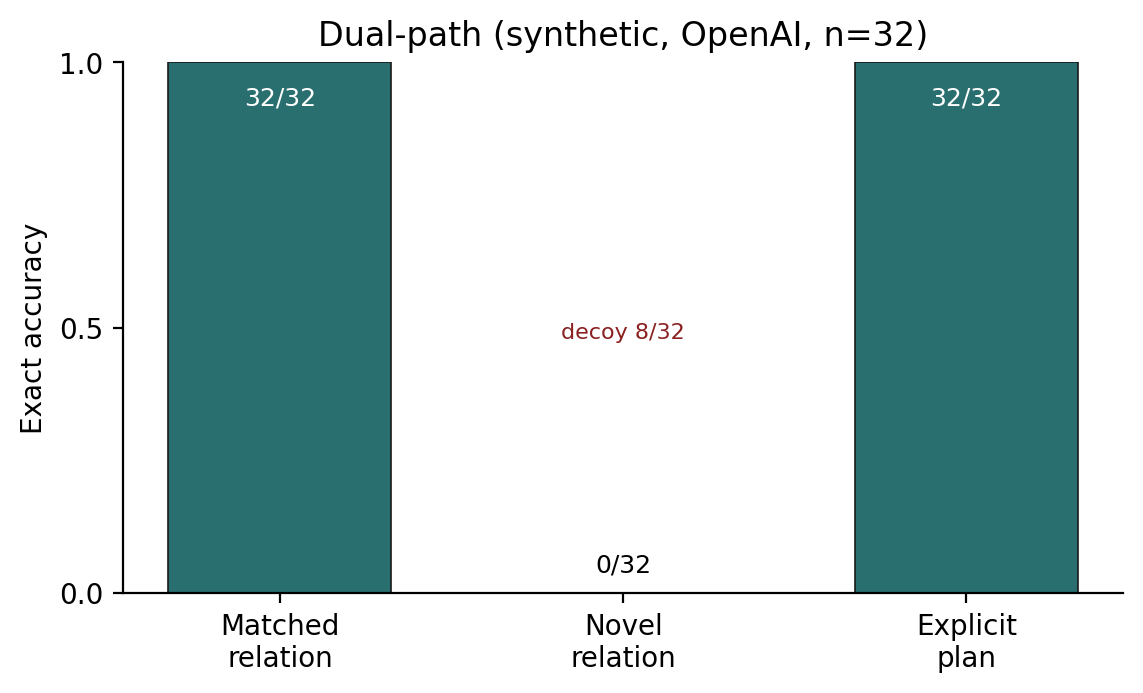
\includegraphics[width=0.72\linewidth]{fig3_dualpath.png}
\caption{\textsc{Dual} (synthetic, OpenAI $n{=}32$): matched $32/32$; novel
$0/32$ (asymmetric decoy $8$); explicit plan $32/32$.}
\label{fig:dualpath}
\end{figure}

An $n{=}8$ cell is zero demos $2/8$; one or more demos $8/8$. Isolation
$n{=}32$ is the reported dual-path measurement.
Local \texttt{mistral}/\texttt{qwen35} runs are not in the roster
(matched-asymmetric $0/32$; Qwen matched-balanced $7/32$; plan n.r.).
Composer isolation-tag novel-relation \texttt{UNKNOWN} is
\texttt{adv\_induction\_n32\_iso\_composer25.json} (helper
\texttt{run\_induce\_mut\_n32\_iso.py}); the free-form lock is
\texttt{composer25ff} (decoy $32/32$). Grok free-form is \texttt{grok45ff}.

\FloatBarrier
\section{No-hop binding (JSON)}
\label{app:ident}

\begin{table}[ht]
\centering
\small
\begin{tabular}{@{}lccc@{}}
\toprule
Arm (no written hop) & OpenAI & Composer~2.5 & Grok~4.5 \\
\midrule
Schema list only & $0/32$ & $0/32$ & $0/32$ \\
English protocol (no hop) & $32/32$ & $32/32$ & $32/32$ \\
Same $\sigma$, silent & $6/32$ & $19/32$ & $31/32$ \\
Same $\sigma$ $+$ equality recipe & $32/32$ & $32/32$ & $32/32$ \\
\texttt{JSONKEY:} match broken & $0/32$ & $0/32$ & $0/32$ \\
Sealed Q, two routes, recipe & $31/32$ & $25/32$ & $32/32$ \\
Sealed Q, two routes, vague hints$^{\ast}$ & $13/32$ & $23/32$ & $31/32$ \\
\bottomrule
\end{tabular}
\caption{Selection support without a written hop (Wikidata CEO JSON; city
or mentor country is the distractor; isolation; per-item HMAC). Schema-only
and broken token overlap fail for all three. An English protocol or an
equality recipe that does not name the field saturates. Silent same-$\sigma$
overlap and vague hints are family-dependent, not a three-family restore.
OpenAI silent $6/32$ and vague-hint $13/32$ include 24 and 15 empty
completions stored as \texttt{UNKNOWN}.
$^{\ast}$Composer vague-hint distractor $1/32$. JOIN was not evaluated at
$n{=}32$. Wilson: $32/32 \Rightarrow [0.89,1.00]$,
$0/32 \Rightarrow [0.00,0.11]$,
$6/32 \Rightarrow [0.09,0.35]$,
$31/32 \Rightarrow [0.84,0.99]$.
Silent same-$\sigma$ OpenAI $6/32$ is a JSON-binding cell, distinct from
\textsc{Wiki-H5}.
\texttt{NS\_SILENT} ARM lines say ``Match impossible''; those $0/32$ rows
are not a sealed-join collapse.}
\label{tab:ident32}
\end{table}

\begin{figure}[ht]
\centering
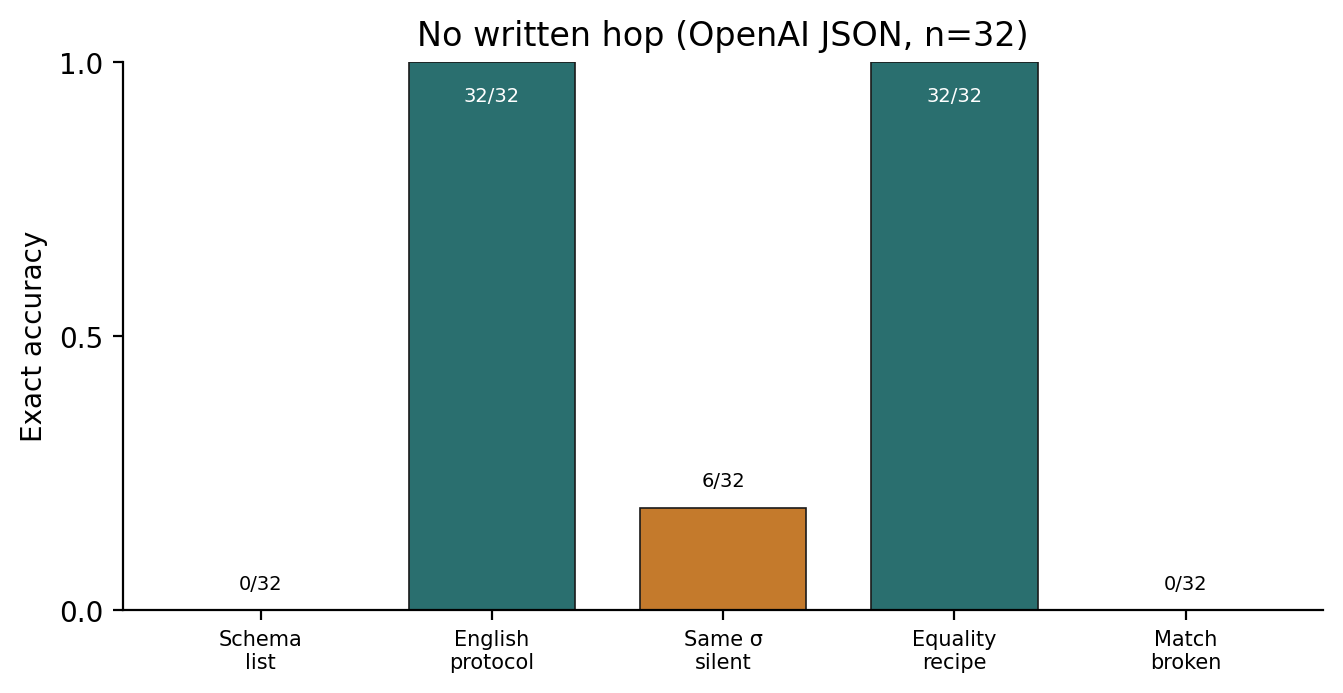
\includegraphics[width=0.92\linewidth]{fig4_binding.png}
\caption{No-hop binding (Wikidata JSON, OpenAI $n{=}32$). Bars are exact
match; the $6/32$ silent bar is gold hits, not a decoy rate.}
\label{fig:bind}
\end{figure}
\FloatBarrier

Figure~\ref{fig:bind} is the OpenAI row of Table~\ref{tab:ident32}.
The Table~\ref{tab:ident32} prompts are fixed English blocks (same wording
for all three families). We use \emph{equality} rather than similarity:
exact identity of sealed tokens, not a continuous metric. Schema list only
is a bilingual \texttt{KEY\_SCHEMA} (\texttt{English name =} sealed JSON
key) plus ``Use the schema to read CONTEXT. No JOIN is given.'' The English
protocol adds that QUESTION and CONTEXT are encoded, that identical tokens
are the same entity or field (equality, not decryption), and that schema
names plus token equality walk CONTEXT; it also names the asked field as
country rather than city. The same-$\sigma$ equality recipe
(Appendix~\ref{app:recipe}) does not name country or city in English. It is
not the \textsc{Wiki-H5} prompt. The suite uses the same 32 Wikidata people
(per-item keys; seed $20260826$--$20260829$).
The OpenAI $n{=}6$ cell with an English question template and English JSON
keys ($1/6$) is not plaintext Wiki-H5: the start token and all values are
sealed, city is a nested distractor under \texttt{hq}, and the prompt
forbids world knowledge and allows \texttt{UNKNOWN}. English keys alone do
not restore the walk.

\section{Sealing middleware}
\label{app:middleware}

The necessary step is binding a typed full name to one graph atom: spaced
tokens otherwise miss $V$. The layer then seals entities, relations, and
sensitive values. When the relation sequence is already specified, the join
can be executed by a deterministic non-LLM router. If the hop is not
compiled, the layer may attach one sealed join as an execution control (not
a list of candidate paths). The model, when used, returns $\sigma(a)$; the
layer unseals. Isolation on the CEO vault without start-entity binding is
$0/6$ vs.\ full layer $6/6$ for Composer~2.5, OpenAI, and an unversioned
Claude endpoint (Anthropic model id not stored; plaintext names in
the packed prompt: $0$). On complex 3-hop and real 2Wiki,
Composer~2.5 without binding is $0/6$ vs.\ layer $6/6$; OpenAI layer $6/6$
(without binding: complex $4/6$, 2Wiki $0/6$). Those isolation files also
attach a join: that is the execution control, not the reason to call a
model. The model never receives a retrieved path list and never answers in
plaintext (Table~\ref{tab:diff}). The $6/6$ scores are this binding-and-join
control, not the free \textsc{Wiki-H5} $6/32$ cell.

\section{Packaging probes}
\label{app:packaging}

These cells test serialization and application packaging. They are
\emph{not} the matched $2{\times}2$, not a second discovery, and not
required to restate the body claim.
Sample sizes are $n{=}6$--$16$ except a counterfactual 2Wiki
sanity check and the public Spider identifier-in-$q$ cell ($n{=}100$).
We keep one paragraph per family so a reader who wants the packaging
inventory can find it; a reader of \textsc{Wiki-H5} can skip this
appendix.

\paragraph{Tables / JSON / SQL / Excel / FinQA / WTQ.}
Same CEO join as markdown tables, nested JSON, or a value store: free
sealed English $0/12$, join plan $12/12$ (Composer~2.5 and OpenAI).
JSON keys without a legend: $0/6$; a key legend yields $6/6$ for
OpenAI only; a join plan yields $6/6$ for both.
Token overlap vs.\ \texttt{SQLCOL:} break on public Spider is
Table~\ref{tab:sqlbind} (OpenAI; identifier-in-$q$ slice $n{=}100$:
$51/100$ vs.\ $0/100$).
Excel NL already names both join predicates (batched $n{=}16$):
Composer $0/16$ (mid-hop error $16/16$) vs.\ plan $16/16$; OpenAI $16/16$
on both.
FinQA / WTQ~\citep{chen2021finqa,pasupat2015wtq} on shared sealed context:
FinQA NL $0/8$ vs.\ gold programs $8/8$; WTQ NL $0/6$ vs.\ LOOKUP DSL
$6/6$ (Composer). OpenAI matches FinQA and WTQ DSL; WTQ NL is $1/6$.
Not a leaderboard.

\paragraph{Counterfactual 2Wiki sanity check.}
Composer~2.5 plain NL $200/200$ (Wikipedia leak $0$); OpenAI batched
$150/200$ with overlap leak $50/200$. We do not treat this as a standard
2Wiki evaluation. Spider: sealed-cell NL $4/12$; model SQL executed locally
$29/32$; gold-SQL engine $191/200$ (Appendix~\ref{app:symbolic}).

\begin{table}[ht]
\centering
\small
\begin{tabular}{@{}lp{7.4cm}@{}}
\toprule
English $q$ & Find the number of papers published by the institution
``University of Pennsylvania''. \\
Sealed $q$ (A) & Find the number of \texttt{E41f626311a9f} published by the
institution ``University of Pennsylvania''. \\
EQ & $q$ token equals sqlite identifier $\to$ execute; first-cell gold on this item \\
NS & same $q$; identifiers are \texttt{HMAC(SQLCOL:name)} $\to$ \texttt{UNKNOWN} \\
\midrule
A (name in $q$) & $n{=}100$ (45 DBs). EQ $51/100$; NS $0/100$ (\texttt{UNKNOWN} $100/100$) \\
B (no name in $q$) & $n{=}26$. EQ $18/26$; NS $20/26$ (English $q$; legend can still bind) \\
\bottomrule
\end{tabular}
\caption{Spider identifier overlap vs.\ namespace break
(OpenAI;~\citealp{yu2018spider}). Slice A $n{=}100$: EQ $51/100$, NS
$0/100$. Not official exact-match. n.r.\ for Composer/Grok.}
\label{tab:sqlbind}
\end{table}

\paragraph{Long context / rename.}
At $\sim$128k and $\sim$1.14M sealed tokens, free sealed NL remains $0/8$;
plans $8/8$. Paired sealed plans under a second HMAC key: $12/12$ with differing
golds (Figure~\ref{fig:rename}).

\begin{figure}[htbp]
\centering
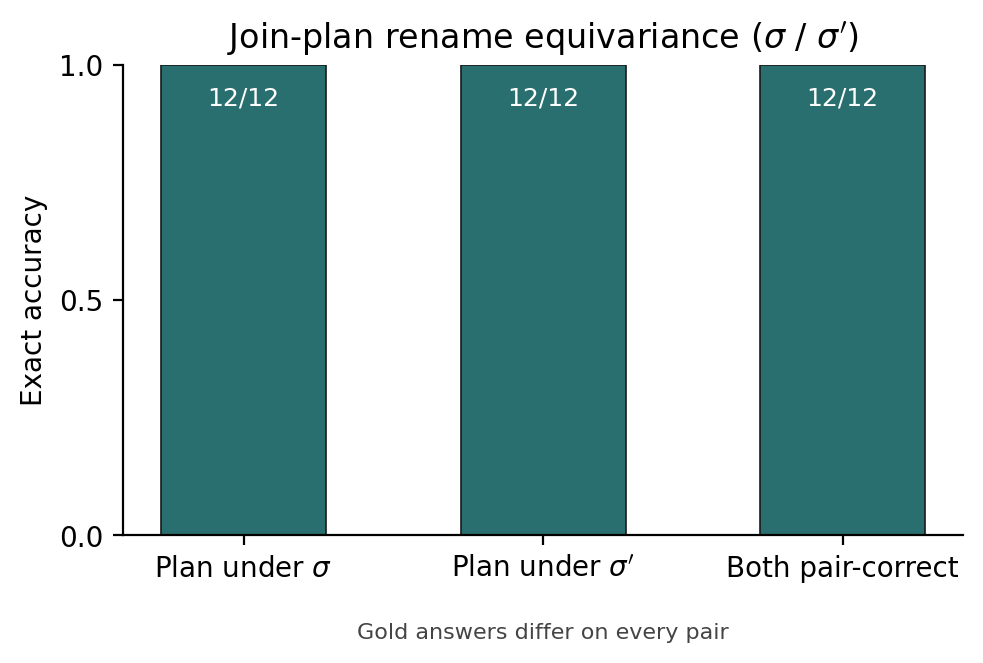
\includegraphics[width=0.88\linewidth]{fig6_rename_equivariance.png}
\caption{Sealed-plan rename equivariance ($n{=}12$): plans remain correct
under a second HMAC key with a different gold on every pair.}
\label{fig:rename}
\end{figure}

\begin{figure}[htbp]
\centering
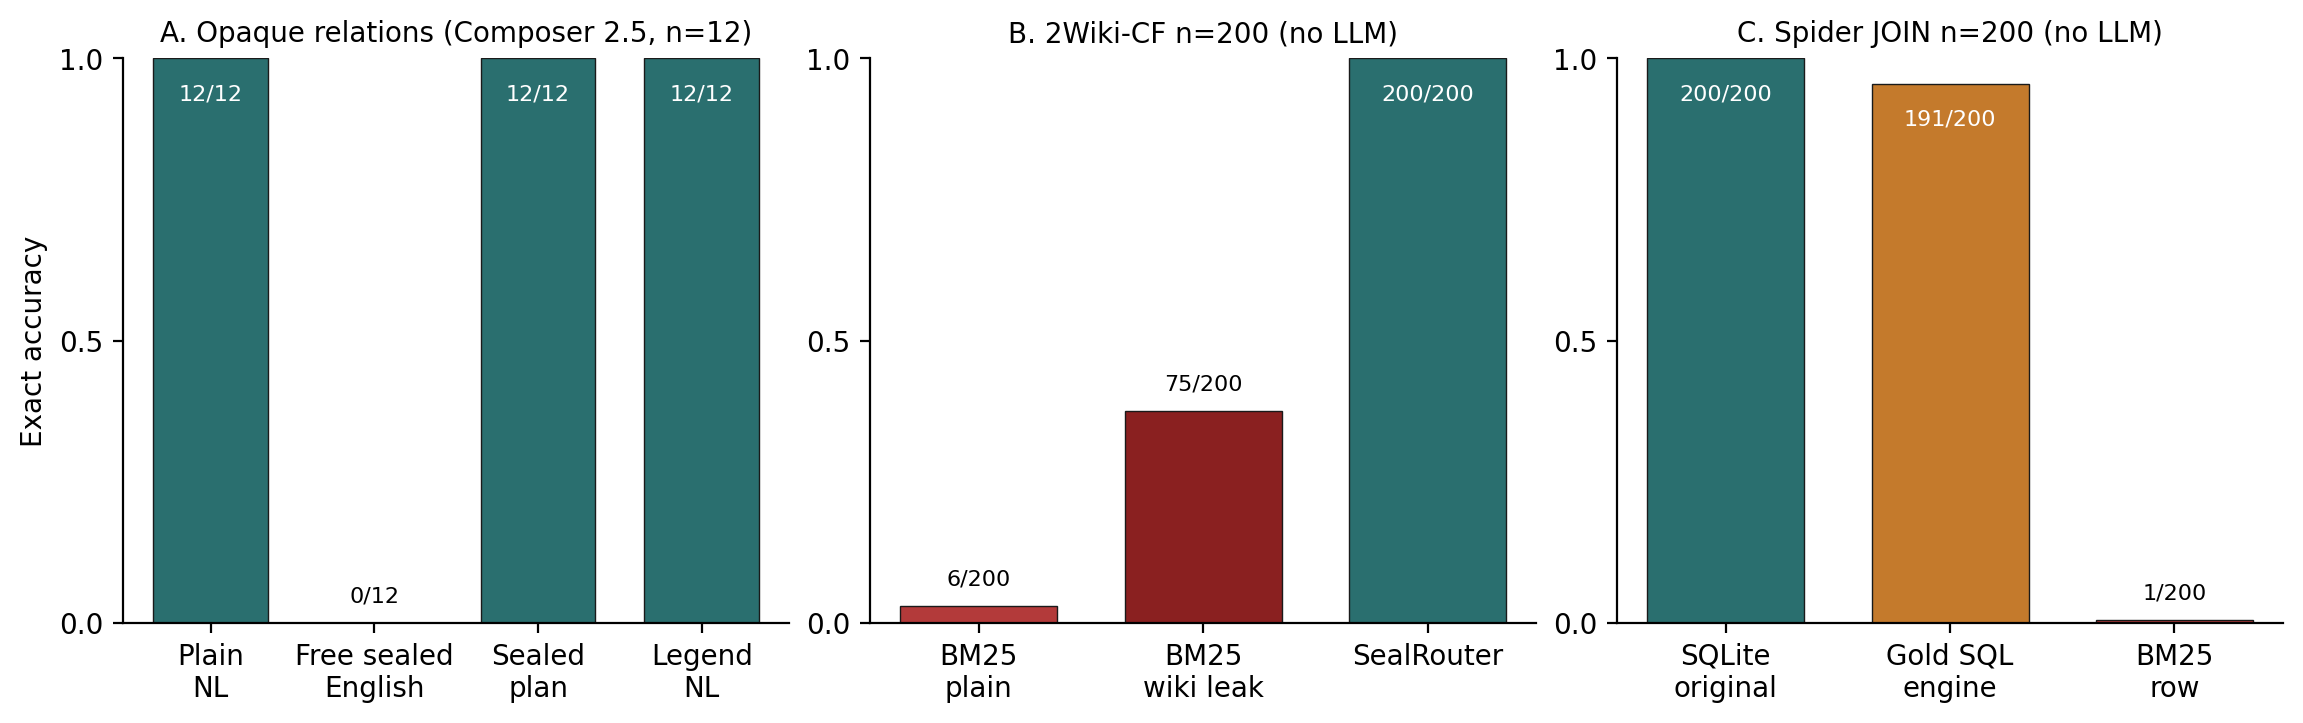
\includegraphics[width=\linewidth]{fig7_opaque_rel_n200.png}
\caption{Non-LLM and packaging controls.
Panel A is Composer $n{=}12$; panels B--C are frozen $n{=}200$ baselines.
Left: plain NL $12/12$, opaque-rel NL $0/12$, plan/legend $12/12$ (Composer~2.5, $n{=}12$).
Middle: 2Wiki-CF BM25 $6/200$, Wikipedia-string leak $75/200$, SealRouter
$200/200$.
Right: Spider sqlite $200/200$, gold-SQL engine $191/200$, BM25 $1/200$.
CEO/2Wiki opacity$\times$prompt-form scores are in the surrounding prose.}
\label{fig:packaging}
\end{figure}

\FloatBarrier
\section{Extended scores}
\label{app:extended}
\label{app:metaqa32}

MetaQA-style 2-hop templates on the same public movie graph are a
question-form control, not an evaluation on the official MetaQA 14K test
split. Plaintext is $32/32$ for all three families. Condition~A (English
question over opaque relations) is OpenAI $32/32$, Composer $19/32$, Grok
$15/32$. Condition~B hashes those verbs except \texttt{[start]}: OpenAI
$25/32$, Composer $27/32$, Grok $14/32$ (plans $32/32$, $31/32$, $32/32$).
That $n{=}32$ template cell is not \textsc{Movie-B}.
Packaging cells with $n{\le}16$ are Appendix~\ref{app:packaging}, not a
second $2{\times}2$.

\section{Sign-flip of the H5 interaction}
\label{app:signflip}

Let $d_i=\mathbf{1}[\text{opaque correct}]-\mathbf{1}[\text{English correct}]$
and $c_i=d^{\mathrm{two}}_i-d^{\mathrm{unique}}_i$.
Of 32 \textsc{Wiki-H5} items, 24 have $c_i{=}{-1}$, one has $c_i{=}{-2}$,
7 have $c_i{=}0$; $T{=}{-}26$.
Under exchangeability of unique-path and two-path opacity effects,
$p{=}2^{-24}{=}5.96{\times}10^{-8}$.
That $p$ coincides numerically with the two-path McNemar $p$ (25 vs.\ 0;
\citealp{mcnemar1947});
the tests are not the same.
Opacity is not a randomized within-item treatment.
The body reports Wilson intervals and the paired counts.

\section{Equality recipe (JSON cell)}
\label{app:recipe}

Verbatim protocol used in Table~\ref{tab:ident32}, \emph{not} in
\textsc{Wiki-H5}:
``QUESTION and CONTEXT use the same encoding. Identical tokens are the same
entity or the same field (equality, not English). START is a QUESTION token
that also appears as an id value in CONTEXT. The asked field is a QUESTION
token that also appears as a JSON key. Walk CONTEXT by token equality.
If more than one reading is possible, UNKNOWN.''

The $n{=}32$ JSON cells are Table~\ref{tab:ident32}. Sample sizes
$n{\le}16$ (vault, Excel, FinQA, WTQ, middleware) are packaging probes
(Appendix~\ref{app:packaging}), not \textsc{Wiki-H5}.

\section{Symbolic execution controls}
\label{app:symbolic}

SealRouter executes a gold sealed path with no LLM. The gold-SQL engine
executes gold Spider SQL locally. Figure~\ref{fig:packaging} summarizes those
controls.

\clearpage
% NeurIPS 2026 Paper Checklist. Do not modify the questions.
% Answers use macros from neurips_2026.sty. Input after the appendix.

\section*{NeurIPS Paper Checklist}

\begin{enumerate}

\item {\bf Claims}
\item[] Question: Do the main claims made in the abstract and introduction accurately reflect the paper's contributions and scope?
\item[] Answer: \answerYes{}
\item[] Justification: The abstract and introduction state a measurement protocol, unique-path sealed traversal, and packaging-sensitive abstention under two competing routes. They report named-arm Wiki-H5 and family$\times$packaging exact-match rates, not a ranking of families, and do not claim a confidentiality proof or a scored $(r_1,r_2)$.
\item[] Guidelines:
\begin{itemize}
\item The answer \answerNA{} means that the abstract and introduction do not include the claims made in the paper.
\item The abstract and/or introduction should clearly state the claims made, including the contributions made in the paper and important assumptions and limitations.
\item The claims made should match theoretical and experimental results, and reflect how much the results can be expected to generalize to other settings.
\item It is fine to include aspirational goals as motivation as long as it is clear that these goals are not attained by the paper.
\end{itemize}

\item {\bf Limitations}
\item[] Question: Does the paper discuss the limitations of the work performed by the authors?
\item[] Answer: \answerYes{}
\item[] Justification: Section~\ref{sec:limitations} states that named-arm Wiki-H5 DiD is most readable for OpenAI, $n{=}32$ on one template (reused on later suites), cyclic decoys, 512 vs.\ 4096/medium packaging, harness mismatch, Dual empty completions, inferred rather than scored $(r_1,r_2)$, OpenAI-only \textsc{Movie-B}/\textsc{Wiki-Shuf}, and controls not evaluated here (forced-choice, short symbols, second seed).
\item[] Guidelines:
\begin{itemize}
\item The answer \answerNA{} means that the paper has no limitation while the answer \answerNo{} means that the paper has limitations, but those are not discussed in the paper.
\item The authors are encouraged to create a separate ``Limitations'' section in their paper.
\item Reviewers are specifically instructed not to penalize honesty concerning limitations.
\end{itemize}

\item {\bf Theory assumptions and proofs}
\item[] Question: For each theoretical result, does the paper provide the full set of assumptions and a complete (and correct) proof?
\item[] Answer: \answerNA{}
\item[] Justification: The paper is a measurement protocol. Section~\ref{sec:problem} defines selection and traversal maps; it does not state theorems.
\item[] Guidelines:
\begin{itemize}
\item The answer \answerNA{} means that the paper does not include theoretical results.
\end{itemize}

\item {\bf Experimental result reproducibility}
\item[] Question: Does the paper fully disclose all the information needed to reproduce the main experimental results of the paper to the extent that it affects the main claims and/or conclusions of the paper (regardless of whether the code and data are provided or not)?
\item[] Answer: \answerYes{}
\item[] Justification: Section~\ref{sec:method} and Appendix~\ref{app:protocol} give seeds, HMAC width, isolation vs.\ batch, scoring (Wiki-H5/Wiki-OO: explicit \texttt{UNKNOWN}; Dual/no-hop OpenAI: empty completions stored as \texttt{UNKNOWN}; new runner: \texttt{NO\_OUTPUT}), model endpoints, and which cells are answer-line locks. Quizzes are in \texttt{runs/}; locked scores in \texttt{results/}.
\item[] Guidelines:
\begin{itemize}
\item The answer \answerNA{} means that the paper does not include experiments.
\item While NeurIPS does not require releasing code, the conference does require all submissions to provide some reasonable avenue for reproducibility.
\end{itemize}

\item {\bf Open access to data and code}
\item[] Question: Does the paper provide open access to the data and code, with sufficient instructions to faithfully reproduce the main experimental results, as described in supplemental material?
\item[] Answer: \answerYes{}
\item[] Justification: Isolation quizzes, locked JSON, reply trees, and \texttt{results/SHA256SUMS} are in the public repository named on the title page. Composer~2.5 and Grok~4.5 used a vendor agent SDK that is not the OpenAI API; Appendix~\ref{app:protocol} records that mismatch.
\item[] Guidelines:
\begin{itemize}
\item The answer \answerNA{} means that the paper does not include experiments requiring code.
\item At submission time, to preserve anonymity, the authors should release anonymized versions (if applicable).
\end{itemize}

\item {\bf Experimental setting/details}
\item[] Question: Does the paper specify all the training and test details (e.g., data splits, hyperparameters, how they were chosen, type of optimizer) necessary to understand the results?
\item[] Answer: \answerYes{}
\item[] Justification: No models are trained. Sampling seed, HMAC keys, $n$, temperature omission, token budgets, and ARM text are in Section~\ref{sec:method} and Appendix~\ref{app:protocol}.
\item[] Guidelines:
\begin{itemize}
\item The answer \answerNA{} means that the paper does not include experiments.
\item The experimental setting should be presented in the core of the paper to a level of detail that is necessary to appreciate the results.
\end{itemize}

\item {\bf Experiment statistical significance}
\item[] Question: Does the paper report error bars suitably and correctly defined or other appropriate information about the statistical significance of the experiments?
\item[] Answer: \answerYes{}
\item[] Justification: Wilson 95\% intervals ($z{=}1.96$) and McNemar exact two-sided complete-case tests are reported for the primary OpenAI $2{\times}2$. Appendix~\ref{app:protocol} notes that cyclic decoys slightly violate the i.i.d.\ assumption of the Wilson intervals.
\item[] Guidelines:
\begin{itemize}
\item The answer \answerNA{} means that the paper does not include experiments.
\item The authors should answer \answerYes{} if the results are accompanied by error bars, confidence intervals, or statistical significance tests, at least for the experiments that support the main claims of the paper.
\end{itemize}

\item {\bf Experiments compute resources}
\item[] Question: For each experiment, does the paper provide sufficient information on the computer resources (type of compute workers, memory, time of execution) needed to reproduce the experiments?
\item[] Answer: \answerYes{}
\item[] Justification: Appendix~\ref{app:protocol} records that no models were trained; OpenAI cells used Chat Completions; Composer/Grok used a hosted agent API; query counts for Wiki-H5 and header$\times$decoy are stated.
\item[] Guidelines:
\begin{itemize}
\item The answer \answerNA{} means that the paper does not include experiments.
\end{itemize}

\item {\bf Code of ethics}
\item[] Question: Does the research conducted in the paper conform, in every respect, with the NeurIPS Code of Ethics \url{https://neurips.cc/public/EthicsGuidelines}?
\item[] Answer: \answerYes{}
\item[] Justification: Instances use licensed public graphs. No human subjects, no crowdwork. Per-item replies are hash-pinned, not a training dump. HMAC is not treated as a privacy mechanism (Ethical considerations).
\item[] Guidelines:
\begin{itemize}
\item The answer \answerNA{} means that the authors have not reviewed the NeurIPS Code of Ethics.
\end{itemize}

\item {\bf Broader impacts}
\item[] Question: Does the paper discuss both potential positive societal impacts and negative societal impacts of the work performed?
\item[] Answer: \answerYes{}
\item[] Justification: Ethical considerations states the diagnostic use and the misuse of reading HMAC seals as confidentiality. The protocol is not a deployed anonymizer.
\item[] Guidelines:
\begin{itemize}
\item The answer \answerNA{} means that there is no societal impact of the work performed.
\end{itemize}

\item {\bf Safeguards}
\item[] Question: Does the paper describe safeguards that have been put in place for responsible release of data or models that have a high risk for misuse (e.g., pre-trained language models, image generators, or scraped datasets)?
\item[] Answer: \answerNA{}
\item[] Justification: The release is quizzes, scores, and hashing code over public KG slices. We do not release pretrained generators or scraped image/text corpora.
\item[] Guidelines:
\begin{itemize}
\item The answer \answerNA{} means that the paper poses no such risks.
\end{itemize}

\item {\bf Licenses for existing assets}
\item[] Question: Are the creators or original owners of assets (e.g., code, data, models), used in the paper, properly credited and are the license and terms of use explicitly mentioned and properly respected?
\item[] Answer: \answerYes{}
\item[] Justification: Wikidata CEO records (CC0), WikiMovies/MetaQA as publicly released (upstream papers do not name a license string), 2WikiMultihopQA (Apache-2.0), and Spider (CC-BY-SA-4.0) are cited in Ethical considerations.
\item[] Guidelines:
\begin{itemize}
\item The answer \answerNA{} means that the paper does not use existing assets.
\item The name of the license (e.g., CC-BY 4.0) should be included for each asset.
\end{itemize}

\item {\bf New assets}
\item[] Question: Are new assets introduced in the paper well documented and is the documentation provided alongside the assets?
\item[] Answer: \answerYes{}
\item[] Justification: Isolation quizzes, locked scores, SHA-256 pins, and per-item reply files are documented in Appendix~\ref{app:protocol} and the repository README. Replies are not released as a training corpus.
\item[] Guidelines:
\begin{itemize}
\item The answer \answerNA{} means that the paper does not release new assets.
\item At submission time, remember to anonymize your assets (if applicable).
\end{itemize}

\item {\bf Crowdsourcing and research with human subjects}
\item[] Question: For crowdsourcing experiments and research with human subjects, does the paper include the full text of instructions given to participants and screenshots, if applicable, as well as details about compensation (if any)?
\item[] Answer: \answerNA{}
\item[] Justification: The study evaluates language-model APIs on public graphs. There are no human participants.
\item[] Guidelines:
\begin{itemize}
\item The answer \answerNA{} means that the paper does not involve crowdsourcing nor research with human subjects.
\end{itemize}

\item {\bf Institutional review board (IRB) approvals or equivalent for research with human subjects}
\item[] Question: Does the paper describe potential risks incurred by study participants, whether such risks were disclosed to the subjects, and whether Institutional Review Board (IRB) approvals (or an equivalent approval/review based on the requirements of your country or institution) were obtained?
\item[] Answer: \answerNA{}
\item[] Justification: No human-subjects research.
\item[] Guidelines:
\begin{itemize}
\item The answer \answerNA{} means that the paper does not involve crowdsourcing nor research with human subjects.
\end{itemize}

\item {\bf Declaration of LLM usage}
\item[] Question: Does the paper describe the usage of LLMs if it is an important, original, or non-standard component of the core methods in this research? Note that if the LLM is used only for writing, editing, or formatting purposes and does not impact the core methodology, scientific rigor, or originality of the research, declaration is not required.
\item[] Answer: \answerNA{}
\item[] Justification: HMAC sealing and the quiz files are the method. Language models are evaluated systems (Section~\ref{sec:method}), not a component of the protocol.
\item[] Guidelines:
\begin{itemize}
\item The answer \answerNA{} means that the core method development in this research does not involve LLMs as any important, original, or non-standard components.
\end{itemize}

\end{enumerate}


\end{document}
